\documentclass[preprint]{sigplanconf}

\usepackage{amssymb}
\usepackage{amsthm}
\usepackage{breakurl}             % Not needed if you use pdflatex only.
\usepackage{color}
\usepackage{epsfig}
\usepackage{esvect}
\usepackage{listings}
\usepackage{mathpartir}
\usepackage{MnSymbol}
\usepackage{multirow}
\usepackage{rotating}

\lstdefinestyle{Caml}{language=Caml,%
  literate={when}{{{\bf when}}}4
}

\lstdefinestyle{C++}{language=C++,%
showstringspaces=false,
  columns=fullflexible,
  escapechar=@,
  basicstyle=\sffamily,
%  commentstyle=\rmfamily\itshape,
  moredelim=**[is][\color{white}]{~}{~},
  literate={[<]}{{\textless}}1      {[>]}{{\textgreater}}1 %
           {<}{{$\langle$}}1        {>}{{$\rangle$}}1 %
           {<=}{{$\leq$}}1          {>=}{{$\geq$}}1          
           {==}{{$==$}}2            {!=}{{$\neq$}}1 %
           {=>}{{$\Rightarrow\;$}}1 {->}{{$\rightarrow{}$}}1 %
           {<:}{{$\subtype{}\ $}}1  {<-}{{$\leftarrow$}}1 %
           {s1;}{{$s_1$;}}3 {s2;}{{$s_2$;}}3 {s3;}{{$s_3$;}}3 {s4;}{{$s_4$;}}3 {s5;}{{$s_5$;}}3 {s6;}{{$s_6$;}}3 {s7;}{{$s_7$;}}3 {sn;}{{$s_n$;}}3 {si;}{{$s_i$;}}3%
           {P1}{{$P_1$}}2 {P2}{{$P_2$}}2 {P3}{{$P_3$}}2 {P4}{{$P_4$}}2 {P5}{{$P_5$}}2 {P6}{{$P_6$}}2 {P7}{{$P_7$}}2 {Pn}{{$P_n$}}2 {Pi}{{$P_i$}}2%
           {D1}{{$D_1$}}2 {D2}{{$D_2$}}2 {D3}{{$D_3$}}2 {D4}{{$D_4$}}2 {D5}{{$D_5$}}2 {D6}{{$D_6$}}2 {D7}{{$D_7$}}2 {Dn}{{$D_n$}}2 {Di}{{$D_i$}}2%
           {e1}{{$e_1$}}2 {e2}{{$e_2$}}2 {e3}{{$e_3$}}2 {e4}{{$e_4$}}2%
           {E1}{{$E_1$}}2 {E2}{{$E_2$}}2 {E3}{{$E_3$}}2 {E4}{{$E_4$}}2%
           {m_e1}{{$m\_e_1$}}4 {m_e2}{{$m\_e_2$}}4 {m_e3}{{$m\_e_3$}}4 {m_e4}{{$m\_e_4$}}4%
           {Divide}{{Divide}}6 %
           {Match}{{\emph{Match}}}5 %
           {Case}{{\emph{Case}}}4 %
           {Que}{{\emph{Que}}}3 %
           {Otherwise}{{\emph{Otherwise}}}9 %
           {EndMatch}{{\emph{EndMatch}}}8 %
           {CM}{{\emph{CM}}}2 {KS}{{\emph{KS}}}2 {KV}{{\emph{KV}}}2 
}
\lstset{style=C++}
\DeclareRobustCommand{\Cpp}{C\texttt{++}}
\DeclareRobustCommand{\code}[1]{{\lstinline[breaklines=false,escapechar=@]{#1}}}
\DeclareRobustCommand{\codebr}[1]{{\lstinline[breaklines=true]{#1}}}
\DeclareRobustCommand{\codehaskell}[1]{{\lstinline[breaklines=false,language=Haskell]{#1}}}
\DeclareRobustCommand{\codeocaml}[1]{{\lstinline[breaklines=false,language=Caml]{#1}}}
\DeclareRobustCommand{\concept}[1]{{\small\textsc{#1}}}
\newcommand{\exclude}[1]{}
\newcommand{\halfline}{\vspace{-1.5ex}}

\newtheorem{lemma}{Lemma}
\newtheorem{theorem}{Theorem}
\newtheorem{corollary}{Corollary}

%% grammar commands
\newcommand{\Rule}[1]{{\rmfamily\itshape{#1}}}
\newcommand{\Alt}{\ensuremath{|}}
\newcommand{\is}{$::=$}
\newcommand{\subtype}{\textless:}
\newcommand{\evals}{\Rightarrow}
\newcommand{\evalspp}{\Rightarrow^+}
\newcommand{\DynCast}[2]{\ensuremath{dc\langle{#1}\rangle({#2})}}
\newcommand{\nullptr}{\ensuremath{\bot}}

\newcommand{\f}[1]{{ {\bf \textcolor{blue}{#1\%}}}}
\newcommand{\s}[1]{{ {\em \textcolor{cyan}{#1\%}}}}
\newcommand{\n}[1]{{ {\bf ~ ~ ~ ~ }}}
\newcommand{\Opn}{{\scriptsize {\bf Open}}}
\newcommand{\Cls}{{\scriptsize {\bf Tag}}}
\newcommand{\Unn}{{\scriptsize {\bf Union}}}

%\newcommand{\gwNGPp}{\n{}}
%\newcommand{\gwNGKp}{\n{}}
 \newcommand{\gwNGUp}{\n{}}
%\newcommand{\gwNSPp}{\n{}}
%\newcommand{\gwNSKp}{\n{}}
 \newcommand{\gwNSUp}{\n{}}
%\newcommand{\vwNGPp}{\n{}}
%\newcommand{\vwNGKp}{\n{}}
 \newcommand{\vwNGUp}{\n{}}
%\newcommand{\vwNSPp}{\n{}}
%\newcommand{\vwNSKp}{\n{}}
 \newcommand{\vwNSUp}{\n{}}
%\newcommand{\vxNGPp}{\n{}}
%\newcommand{\vxNGKp}{\n{}}
 \newcommand{\vxNGUp}{\n{}}
%\newcommand{\vxNSPp}{\n{}}
%\newcommand{\vxNSKp}{\n{}}
 \newcommand{\vxNSUp}{\n{}}

%\newcommand{\gwNGPq}{\n{}}
%\newcommand{\gwNGKq}{\n{}}
 \newcommand{\gwNGUq}{\n{}}
%\newcommand{\gwNSPq}{\n{}}
%\newcommand{\gwNSKq}{\n{}}
 \newcommand{\gwNSUq}{\n{}}
%\newcommand{\vwNGPq}{\n{}}
%\newcommand{\vwNGKq}{\n{}}
 \newcommand{\vwNGUq}{\n{}}
%\newcommand{\vwNSPq}{\n{}}
%\newcommand{\vwNSKq}{\n{}}
 \newcommand{\vwNSUq}{\n{}}
%\newcommand{\vxNGPq}{\n{}}
%\newcommand{\vxNGKq}{\n{}}
 \newcommand{\vxNGUq}{\n{}}
%\newcommand{\vxNSPq}{\n{}}
%\newcommand{\vxNSKq}{\n{}}
 \newcommand{\vxNSUq}{\n{}}

%\newcommand{\gwNGPn}{\n{}}
%\newcommand{\gwNGKn}{\n{}}
 \newcommand{\gwNGUn}{\n{}}
%\newcommand{\gwNSPn}{\n{}}
%\newcommand{\gwNSKn}{\n{}}
 \newcommand{\gwNSUn}{\n{}}
%\newcommand{\vwNGPn}{\n{}}
%\newcommand{\vwNGKn}{\n{}}
 \newcommand{\vwNGUn}{\n{}}
%\newcommand{\vwNSPn}{\n{}}
%\newcommand{\vwNSKn}{\n{}}
 \newcommand{\vwNSUn}{\n{}}
%\newcommand{\vxNGPn}{\n{}}
%\newcommand{\vxNGKn}{\n{}}
 \newcommand{\vxNGUn}{\n{}}
%\newcommand{\vxNSPn}{\n{}}
%\newcommand{\vxNSKn}{\n{}}
 \newcommand{\vxNSUn}{\n{}}


%\newcommand{\gwYGPp}{\n{}}
% \newcommand{\gwYGKp}{\n{}}
 \newcommand{\gwYGUp}{\n{}}
%\newcommand{\gwYSPp}{\n{}}
% \newcommand{\gwYSKp}{\n{}}
 \newcommand{\gwYSUp}{\n{}}
%\newcommand{\vwYGPp}{\n{}}
% \newcommand{\vwYGKp}{\n{}}
 \newcommand{\vwYGUp}{\n{}}
%\newcommand{\vwYSPp}{\n{}}
% \newcommand{\vwYSKp}{\n{}}
 \newcommand{\vwYSUp}{\n{}}
%\newcommand{\vxYGPp}{\n{}}
% \newcommand{\vxYGKp}{\n{}}
 \newcommand{\vxYGUp}{\n{}}
%\newcommand{\vxYSPp}{\n{}}
% \newcommand{\vxYSKp}{\n{}}
 \newcommand{\vxYSUp}{\n{}}

%\newcommand{\gwYGPq}{\n{}}
% \newcommand{\gwYGKq}{\n{}}
 \newcommand{\gwYGUq}{\n{}}
%\newcommand{\gwYSPq}{\n{}}
% \newcommand{\gwYSKq}{\n{}}
 \newcommand{\gwYSUq}{\n{}}
%\newcommand{\vwYGPq}{\n{}}
% \newcommand{\vwYGKq}{\n{}}
 \newcommand{\vwYGUq}{\n{}}
%\newcommand{\vwYSPq}{\n{}}
% \newcommand{\vwYSKq}{\n{}}
 \newcommand{\vwYSUq}{\n{}}
%\newcommand{\vxYGPq}{\n{}}
% \newcommand{\vxYGKq}{\n{}}
 \newcommand{\vxYGUq}{\n{}}
%\newcommand{\vxYSPq}{\n{}}
% \newcommand{\vxYSKq}{\n{}}
 \newcommand{\vxYSUq}{\n{}}

%\newcommand{\gwYGPn}{\n{}}
% \newcommand{\gwYGKn}{\n{}}
 \newcommand{\gwYGUn}{\n{}}
%\newcommand{\gwYSPn}{\n{}}
% \newcommand{\gwYSKn}{\n{}}
 \newcommand{\gwYSUn}{\n{}}
%\newcommand{\vwYGPn}{\n{}}
% \newcommand{\vwYGKn}{\n{}}
 \newcommand{\vwYGUn}{\n{}}
%\newcommand{\vwYSPn}{\n{}}
% \newcommand{\vwYSKn}{\n{}}
 \newcommand{\vwYSUn}{\n{}}
%\newcommand{\vxYGPn}{\n{}}
% \newcommand{\vxYGKn}{\n{}}
 \newcommand{\vxYGUn}{\n{}}
%\newcommand{\vxYSPn}{\n{}}
% \newcommand{\vxYSKn}{\n{}}
 \newcommand{\vxYSUn}{\n{}}

 \newcommand{\GwNGPp}{\n{}}
 \newcommand{\GwNGKp}{\n{}}
 \newcommand{\GwNGUp}{\n{}}
 \newcommand{\GwNSPp}{\n{}}
 \newcommand{\GwNSKp}{\n{}}
 \newcommand{\GwNSUp}{\n{}}
%\newcommand{\VwNGPp}{\n{}}
%\newcommand{\VwNGKp}{\n{}}
 \newcommand{\VwNGUp}{\n{}}
%\newcommand{\VwNSPp}{\n{}}
%\newcommand{\VwNSKp}{\n{}}
 \newcommand{\VwNSUp}{\n{}}
%\newcommand{\VxNGPp}{\n{}}
%\newcommand{\VxNGKp}{\n{}}
 \newcommand{\VxNGUp}{\n{}}
%\newcommand{\VxNSPp}{\n{}}
%\newcommand{\VxNSKp}{\n{}}
 \newcommand{\VxNSUp}{\n{}}

 \newcommand{\GwNGPq}{\n{}}
 \newcommand{\GwNGKq}{\n{}}
 \newcommand{\GwNGUq}{\n{}}
 \newcommand{\GwNSPq}{\n{}}
 \newcommand{\GwNSKq}{\n{}}
 \newcommand{\GwNSUq}{\n{}}
%\newcommand{\VwNGPq}{\n{}}
%\newcommand{\VwNGKq}{\n{}}
 \newcommand{\VwNGUq}{\n{}}
%\newcommand{\VwNSPq}{\n{}}
%\newcommand{\VwNSKq}{\n{}}
 \newcommand{\VwNSUq}{\n{}}
%\newcommand{\VxNGPq}{\n{}}
%\newcommand{\VxNGKq}{\n{}}
 \newcommand{\VxNGUq}{\n{}}
%\newcommand{\VxNSPq}{\n{}}
%\newcommand{\VxNSKq}{\n{}}
 \newcommand{\VxNSUq}{\n{}}

 \newcommand{\GwNGPn}{\n{}}
 \newcommand{\GwNGKn}{\n{}}
 \newcommand{\GwNGUn}{\n{}}
 \newcommand{\GwNSPn}{\n{}}
 \newcommand{\GwNSKn}{\n{}}
 \newcommand{\GwNSUn}{\n{}}
%\newcommand{\VwNGPn}{\n{}}
%\newcommand{\VwNGKn}{\n{}}
 \newcommand{\VwNGUn}{\n{}}
%\newcommand{\VwNSPn}{\n{}}
%\newcommand{\VwNSKn}{\n{}}
 \newcommand{\VwNSUn}{\n{}}
%\newcommand{\VxNGPn}{\n{}}
%\newcommand{\VxNGKn}{\n{}}
 \newcommand{\VxNGUn}{\n{}}
%\newcommand{\VxNSPn}{\n{}}
%\newcommand{\VxNSKn}{\n{}}
 \newcommand{\VxNSUn}{\n{}}


 \newcommand{\GwYGPp}{\n{}}
 \newcommand{\GwYGKp}{\n{}}
 \newcommand{\GwYGUp}{\n{}}
 \newcommand{\GwYSPp}{\n{}}
 \newcommand{\GwYSKp}{\n{}}
 \newcommand{\GwYSUp}{\n{}}
%\newcommand{\VwYGPp}{\n{}}
% \newcommand{\VwYGKp}{\n{}}
 \newcommand{\VwYGUp}{\n{}}
%\newcommand{\VwYSPp}{\n{}}
% \newcommand{\VwYSKp}{\n{}}
 \newcommand{\VwYSUp}{\n{}}
%\newcommand{\VxYGPp}{\n{}}
% \newcommand{\VxYGKp}{\n{}}
 \newcommand{\VxYGUp}{\n{}}
%\newcommand{\VxYSPp}{\n{}}
% \newcommand{\VxYSKp}{\n{}}
 \newcommand{\VxYSUp}{\n{}}

 \newcommand{\GwYGPq}{\n{}}
 \newcommand{\GwYGKq}{\n{}}
 \newcommand{\GwYGUq}{\n{}}
 \newcommand{\GwYSPq}{\n{}}
 \newcommand{\GwYSKq}{\n{}}
 \newcommand{\GwYSUq}{\n{}}
%\newcommand{\VwYGPq}{\n{}}
% \newcommand{\VwYGKq}{\n{}}
 \newcommand{\VwYGUq}{\n{}}
%\newcommand{\VwYSPq}{\n{}}
% \newcommand{\VwYSKq}{\n{}}
 \newcommand{\VwYSUq}{\n{}}
%\newcommand{\VxYGPq}{\n{}}
% \newcommand{\VxYGKq}{\n{}}
 \newcommand{\VxYGUq}{\n{}}
%\newcommand{\VxYSPq}{\n{}}
% \newcommand{\VxYSKq}{\n{}}
 \newcommand{\VxYSUq}{\n{}}

 \newcommand{\GwYGPn}{\n{}}
 \newcommand{\GwYGKn}{\n{}}
 \newcommand{\GwYGUn}{\n{}}
 \newcommand{\GwYSPn}{\n{}}
 \newcommand{\GwYSKn}{\n{}}
 \newcommand{\GwYSUn}{\n{}}
%\newcommand{\VwYGPn}{\n{}}
% \newcommand{\VwYGKn}{\n{}}
 \newcommand{\VwYGUn}{\n{}}
%\newcommand{\VwYSPn}{\n{}}
% \newcommand{\VwYSKn}{\n{}}
 \newcommand{\VwYSUn}{\n{}}
%\newcommand{\VxYGPn}{\n{}}
% \newcommand{\VxYGKn}{\n{}}
 \newcommand{\VxYGUn}{\n{}}
%\newcommand{\VxYSPn}{\n{}}
% \newcommand{\VxYSKn}{\n{}}
 \newcommand{\VxYSUn}{\n{}}

% This file defines variables with performance numbers for the table in Evaluation section
% Data from 2011-08-30 
\newcommand{\vwYGKp}{\s{3}}
\newcommand{\vwYGKn}{\s{8}}
\newcommand{\vwYGKq}{\s{11}}
\newcommand{\vwYGPp}{\f{10}}
\newcommand{\vwYGPn}{\f{14}}
\newcommand{\vwYGPq}{\s{0}}
\newcommand{\vwYSKp}{\s{7}}
\newcommand{\vwYSKn}{\s{7}}
\newcommand{\vwYSKq}{\s{10}}
\newcommand{\vwYSPp}{\f{10}}
\newcommand{\vwYSPn}{\f{14}}
\newcommand{\vwYSPq}{\s{0}}
\newcommand{\vwNGKp}{\f{35}}
\newcommand{\vwNGKn}{\s{6}}
\newcommand{\vwNGKq}{\s{5}}
\newcommand{\vwNGPp}{\f{1}}
\newcommand{\vwNGPn}{\s{1}}
\newcommand{\vwNGPq}{\s{10}}
\newcommand{\vwNSKp}{\f{133}}
\newcommand{\vwNSKn}{\f{25}}
\newcommand{\vwNSKq}{\f{59}}
\newcommand{\vwNSPp}{\f{1}}
\newcommand{\vwNSPn}{\s{1}}
\newcommand{\vwNSPq}{\s{8}}

\newcommand{\vxYGKp}{\s{61}}
\newcommand{\vxYGKn}{\s{24}}
\newcommand{\vxYGKq}{\s{25}}
\newcommand{\vxYGPp}{\s{24}}
\newcommand{\vxYGPn}{\s{24}}
\newcommand{\vxYGPq}{\s{36}}
\newcommand{\vxYSKp}{\s{79}}
\newcommand{\vxYSKn}{\s{25}}
\newcommand{\vxYSKq}{\s{35}}
\newcommand{\vxYSPp}{\s{9}}
\newcommand{\vxYSPn}{\s{23}}
\newcommand{\vxYSPq}{\f{133}}
\newcommand{\vxNGKp}{\s{8}}
\newcommand{\vxNGKn}{\s{5}}
\newcommand{\vxNGKq}{\s{0}}
\newcommand{\vxNGPp}{\s{33}}
\newcommand{\vxNGPn}{\s{47}}
\newcommand{\vxNGPq}{\s{43}}
\newcommand{\vxNSKp}{\f{38}}
\newcommand{\vxNSKn}{\f{12}}
\newcommand{\vxNSKq}{\f{3}}
\newcommand{\vxNSPp}{\s{27}}
\newcommand{\vxNSPn}{\s{44}}
\newcommand{\vxNSPq}{\s{45}}

\newcommand{\gwYGKp}{\f{88}}
\newcommand{\gwYGKn}{\f{32}}
\newcommand{\gwYGKq}{\f{250}}
\newcommand{\gwYGPp}{\f{67}}
\newcommand{\gwYGPn}{\f{28}}
\newcommand{\gwYGPq}{\f{87}}
\newcommand{\gwYSKp}{\f{79}}
\newcommand{\gwYSKn}{\f{31}}
\newcommand{\gwYSKq}{\f{259}}
\newcommand{\gwYSPp}{\f{67}}
\newcommand{\gwYSPn}{\f{27}}
\newcommand{\gwYSPq}{\f{90}}
\newcommand{\gwNGKp}{\f{116}}
\newcommand{\gwNGKn}{\f{29}}
\newcommand{\gwNGKq}{\f{43}}
\newcommand{\gwNGPp}{\f{55}}
\newcommand{\gwNGPn}{\s{0}}
\newcommand{\gwNGPq}{\f{1}}
\newcommand{\gwNSKp}{\f{216}}
\newcommand{\gwNSKn}{\f{542}}
\newcommand{\gwNSKq}{\f{520}}
\newcommand{\gwNSPp}{\f{55}}
\newcommand{\gwNSPn}{\f{1}}
\newcommand{\gwNSPq}{\f{3}}

\newcommand{\VwYGKp}{\f{16}}
\newcommand{\VwYGKn}{\f{11}}
\newcommand{\VwYGKq}{\f{168}}
\newcommand{\VwYGPp}{\f{10}}
\newcommand{\VwYGPn}{\f{19}}
\newcommand{\VwYGPq}{\f{153}}
\newcommand{\VwYSKp}{\f{31}}
\newcommand{\VwYSKn}{\f{24}}
\newcommand{\VwYSKq}{\f{185}}
\newcommand{\VwYSPp}{\f{10}}
\newcommand{\VwYSPn}{\f{18}}
\newcommand{\VwYSPq}{\f{153}}
\newcommand{\VwNGKp}{\f{61}}
\newcommand{\VwNGKn}{\f{18}}
\newcommand{\VwNGKq}{\f{13}}
\newcommand{\VwNGPp}{\f{4}}
\newcommand{\VwNGPn}{\s{17}}
\newcommand{\VwNGPq}{\s{9}}
\newcommand{\VwNSKp}{\f{124}}
\newcommand{\VwNSKn}{\f{43}}
\newcommand{\VwNSKq}{\f{34}}
\newcommand{\VwNSPp}{\f{4}}
\newcommand{\VwNSPn}{\s{18}}
\newcommand{\VwNSPq}{\f{3}}
               
\newcommand{\VxYGKp}{\s{5}}
\newcommand{\VxYGKn}{\s{2}}
\newcommand{\VxYGKq}{\f{132}}
\newcommand{\VxYGPp}{\s{5}}
\newcommand{\VxYGPn}{\s{5}}
\newcommand{\VxYGPq}{\f{130}}
\newcommand{\VxYSKp}{\s{9}}
\newcommand{\VxYSKn}{\s{10}}
\newcommand{\VxYSKq}{\f{118}}
\newcommand{\VxYSPp}{\s{6}}
\newcommand{\VxYSPn}{\s{6}}
\newcommand{\VxYSPq}{\f{145}}
\newcommand{\VxNGKp}{\f{20}}
\newcommand{\VxNGKn}{\f{7}}
\newcommand{\VxNGKq}{\f{34}}
\newcommand{\VxNGPp}{\s{14}}
\newcommand{\VxNGPn}{\s{27}}
\newcommand{\VxNGPq}{\f{2}}
\newcommand{\VxNSKp}{\f{47}}
\newcommand{\VxNSKn}{\f{16}}
\newcommand{\VxNSKq}{\f{14}}
\newcommand{\VxNSPp}{\s{0}}
\newcommand{\VxNSPn}{\s{27}}
\newcommand{\VxNSPq}{\f{1}}


\newsavebox{\sembox}
\newlength{\semwidth}
\newlength{\boxwidth}

\newcommand{\Sem}[1]{%
\sbox{\sembox}{\ensuremath{#1}}%
\settowidth{\semwidth}{\usebox{\sembox}}%
\sbox{\sembox}{\ensuremath{\left[\usebox{\sembox}\right]}}%
\settowidth{\boxwidth}{\usebox{\sembox}}%
\addtolength{\boxwidth}{-\semwidth}%
\left[\hspace{-0.3\boxwidth}%
\usebox{\sembox}%
\hspace{-0.3\boxwidth}\right]%
}

\newcommand{\authormodification}[2]{{\color{#1}#2}}
\newcommand{\ys}[1]{\authormodification{blue}{#1}}
\newcommand{\bs}[1]{\authormodification{red}{#1}}
\newcommand{\gdr}[1]{\authormodification{magenta}{#1}}

\begin{document}

%\conferenceinfo{PLDI 2012}{Beijing, China} 
%\copyrightyear{2012} 
%\copyrightdata{[to be supplied]} 

\titlebanner{Draft}        % These are ignored unless
\preprintfooter{Y.Solodkyy, G.Dos Reis, B.Stroustrup: Efficient Type Switch for Object-Oriented Languages}   % 'preprint' option specified.

\title{Efficient Type Switch for Object-Oriented Languages}
%\subtitle{your \code{visit}, Jim, is not \code{accept}able anymore}
%\subtitle{\code{accepting} aint no \code{visit}ors}

\authorinfo{Yuriy Solodkyy\and Gabriel Dos Reis\and Bjarne Stroustrup}
           {Texas A\&M University\\ Texas, USA}
           {\{yuriys,gdr,bs\}@cse.tamu.edu}

\maketitle

\begin{abstract}
We present techniques that can be used in a compiler and/or library setting to 
implement efficiently type switching, type testing, pattern matching, predicate 
dispatch, multi-methods and other facilities that depend on run-time type of the 
argument. The techniques cope well with multiple inheritance in C++, however 
they are not specific to C++ and can be adapted to implementation of similar 
facilities in other languages.

Our library-only implementation of a type switch based on these techniques, equals 
or outperforms visitor design pattern, as commonly used for type-casing 
scenarios in C++, and for many use cases, it equals or outperforms equivalent 
code in languages with built-in type switching constructs. While remaining a 
library-only solution, such a facility better addresses expression problem 
than the visitor design pattern does: it is non-intrusive and does not have 
extensibility restrictions. It also avoids control inversion characteristic to 
visitors, making the code significantly more concise and easier to comprehend.
The library was motivated by and is used for applications involving large, 
typed, abstract syntax trees.
\end{abstract}

\category{CR-number}{subcategory}{third-level}

\terms
Languages, Design

\keywords
Pattern Matching, Visitor Design Pattern, Expression Problem, C++

\section{Introduction} %%%%%%%%%%%%%%%%%%%%%%%%%%%%%%%%%%%%%%%%%%%%%%%%%%%%%%%%%
\label{sec:intro}

%Motivate the problem
%Give a summary of the paper: what you did and how
%Explicitly state your contribution

%Expression problem is a problem of supporting in a programming language modular 
%extensibility of both data and functions at the same time. Functional languages
%allow for easy addition of new functions at the expense of disallowing new data
%variants. Object-oriented languages allow for easy addition of new variants at 
%the expense of disallowing new functions. Many attempts have been made to 
%resolve this dilema in both camps, nevertheless no universally accepted solution 
%that is modular, open and efficient has been found.

%Visitor Design Pattern has became de-facto standard in dealing with expression 
%problem in many industry-strength object-oriented languages because of two 
%factors: its speed and being a library solution. It comes at the cost of 
%restricting extensibility of data, increased verbosity and being hard to teach 
%and understand, but nevertheless, remains the weapon of choice for interacting 
%with numerous object-oriented libraries and frameworks. 

%\subsection{Expression Problem}
%\label{sec:exp}

Functional languages allow for easy addition of new functions on existing data 
types, but fall short in extending data types themselves (e.g. with new constructors), 
which requires modifying the source code. Object-oriented languages, on the 
other hand, make data type extension trivial through inheritance, but addition 
of new functions that work on these classes typically requires changes to class 
definition. This dilemma was first discussed by Cook\cite{Cook90} and then 
accentuated by Wadler\cite{exprproblem} under the name \emph{expression problem} 
he coined. Quoting Wadler:

\emph{``The Expression Problem is a new name for an old problem. The goal is
to define a datatype by cases, where one can add new cases to the
datatype and new functions over the datatype, without recompiling
existing code, and while retaining static type safety (e.g., no
casts)''}.

Zenger and Odersky later refined the problem in the context of independently 
extensible solutions\cite{fool12} as a challenge to find an implementation 
technique, which satisfies the following requirements:

\begin{itemize}
\setlength{\itemsep}{0pt}
\setlength{\parskip}{0pt}
\item {\bf Extensibility in both dimensions}: It should be possible to add new 
      data variants, while adapting the existing operations accordingly. It 
      should also be possible to introduce new functions. 
\item {\bf Strong static type safety}: It should be impossible to apply a 
      function to a data variant, which it cannot handle. 
\item {\bf No modification or duplication}: Existing code should neither be 
      modified nor duplicated.
\item {\bf Separate compilation}: Neither datatype extensions nor addition of 
      new functions should require re-typechecking the original datatype or 
      existing functions. No safety checks should be deferred until link or 
      runtime.
\item {\bf Independent extensibility}: It should be possible to combine 
      independently developed extensions so that they can be used jointly.
\end{itemize}

%Paraphrasing, the expression problem can be summarized as a problem of 
%supporting modular extensibility of both data and functions at the same time in 
%one programming language.

\noindent
Object-oriented languages further complicate the matter with the fact that 
data variants may form subtyping relationship between themselves, which made us 
introduce an additional requirement:

\begin{itemize}
\setlength{\itemsep}{0pt}
\setlength{\parskip}{0pt}
\item {\bf Substitutability}: Operations expressed on more general data variants
      should be applicable to more specific ones that are in subtyping relation 
      with them.
\end{itemize}

%Depending on the semantics of the language's subtyping relation, 
%substitutability requirement may turn pattern matching into an expensive 
%operation. OCaml, for example, that uses structural subtyping on its object 
%types, does not offer pattern 

\noindent
Numerous solutions have been proposed to dealing with expression problem in both 
functional and object-oriented camps, but notably very few satisfy all of the 
above requirements, while none has made its way into one of the mainstream 
languages. We refer the reader to Zenger and Odersky's original  
manuscript for discussion of the approaches\cite{fool12}. Interestingly, most of 
the discussed object-oriented solutions were focusing on the visitor design 
pattern\cite{DesignPatterns1993}, which even today seems to be the most commonly 
used approach to dealing with the expression problem in practice.

\subsection{Visitor Design Pattern}
\label{sec:vdp}

%Discuss visitor design pattern and its problems.
%\begin{itemize}
%\item Intrusive - requires changes to the hierarchy
%\item Not open  - addition of new classes changes visitor interface
%\item Does not provide by default relation between visitors of base and derived classes
%\item Control inversion
%\item Cannot be generically extended to handling n arguments
%\end{itemize}

\emph{Visitor Design Pattern}\cite{DesignPatterns1993} was devised to solve a problem 
of extending existing classes with new functions in object-oriented languages. 
Consider for example a simple language of expressions:

\begin{lstlisting}
@$exp$ \is{} $val$ \Alt{} $exp+exp$ \Alt{} $exp-exp$ \Alt{} $exp*exp$ \Alt{} $exp/exp$@
\end{lstlisting}

\noindent
OCaml data type describing this grammar as well as simple evaluator of expressions 
in it can be declared as following:

\begin{lstlisting}[language=Caml,keepspaces,columns=flexible]
type expr = Value of int 
          | Plus  of expr * expr | Minus  of expr * expr 
          | Times of expr * expr | Divide of expr * expr
          ;;

let rec eval e =
  match e with
            Value  v      -> v
          | Plus   (a, b) -> (eval a) + (eval b)
          | Minus  (a, b) -> (eval a) - (eval b)
          | Times  (a, b) -> (eval a) * (eval b)
          | Divide (a, b) -> (eval a) / (eval b)
          ;;
\end{lstlisting}

\noindent
The corresponding C++ data types would most likely be parameterized, but for
now we will just use simple classes:

\begin{lstlisting}[keepspaces,columns=flexible]
struct Expr { virtual @$\sim$@Expr() {} };
struct Value  : Expr { int value; };
struct Plus   : Expr { Expr* exp1; Expr* exp2; };
struct Minus  : Expr { Expr* exp1; Expr* exp2; };
struct Times  : Expr { Expr* exp1; Expr* exp2; };
struct Divide : Expr { Expr* exp1; Expr* exp2; };
\end{lstlisting}

\noindent
A similar evaluator can be implemented with a virtual function \code{virtual int 
eval() const = 0;} declared in the \code{Expr} class. The function is overridden 
in each of the derived classes to handle corresponding case, e.g.:

\begin{lstlisting}[keepspaces,columns=flexible]
int Value::eval() const { return value; }
int Times::eval() const { return exp1->eval()*exp2->eval(); }
\end{lstlisting}

\noindent
Imagine, however, that besides evaluation we would like to provide a pretty 
printing of expressions. A typical object-oriented approach would be to 
introduce a virtual function \\ \code{virtual void print() const = 0;} inside 
the abstract base class \code{Expr}, which will be implemented correspondingly 
in all the derived classes. This works well as long as we know all the required  
operations on the abstract class in advance. Unfortunately, this is very 
difficult to achieve in reality as the code evolves, especially in production 
environment. To put this in context, imagine that after the above interface with 
pretty printing functionality has been deployed, we decided that we need a 
similar functionality that saves the expression in XML format. Adding new 
virtual function implies modifying the base class and creating a versioning 
problem with the code that has been deployed already using the old interface.

To alleviate this problem, the Visitor Design Pattern separates the 
\emph{commonality} of all such future member-functions from their 
\emph{specifics}. The former deals with identifying the most specific derived 
class of the receiver object, known to the system at the time the base class was 
designed. The latter provides implementation of the required functionality once 
the most specific derived class has been identified. The interaction between the 
two is encoded in the protocol that fixes a \emph{visitation interface} 
enumerating all known derived classes on one side and a dispatching mechanism 
that guarantees to select the most specific case with respect to the dynamic 
type of the receiver in the visitation interface. An implementation of this 
protocol for our Expr example might look as following:

\begin{lstlisting}
struct Value; struct Plus; ... struct Divide;
@\halfline@
struct ExprVisitor { // Visitation interface
    virtual void visit(const Value&)  = 0;
    ...  // One virtual function per each known derived class
    virtual void visit(const Divide&) = 0;
};
@\halfline@
struct Expr { // Abstract base
    virtual void accept(ExprVisitor&) const = 0; };
struct Value : Expr { ... // Known derived classes
    void accept(ExprVisitor& v) const { v.visit(*this); } };
\end{lstlisting}

\noindent
Note that even though implementations of \code{accept} member-functions in all 
derived classes are syntactically identical, a different \code{visit} is called. 
We rely here on the overload resolution mechanism of C++ to pick the most 
specialized \code{visit} member-function applicable to the static type of 
\code{*this}.

%This mere code 
%maintenance convenience unfortunately, often confuses novices on what 
%is going on. We thus would like to point out that member-functions in the 
%visitation interface are not required to be called with the same name, -- we 
%could have equally well called them \code{visit_value}, \code{visit_plus} etc. 
%making the corresponding changes to calls inside \code{Value::accept}, 
%\code{Plus::accept} etc.

A user can now implement new functions by overriding \code{ExprVisitor}'s 
functions. For example:

\begin{lstlisting}
std::string to_str(const Expr* e) // Converts expressions to string
{
  struct ToStrVisitor : ExprVisitor
  {
    void visit(const Value& e) { result = std::to_string(e.value); }
    ...
    void visit(const Divide& e) { 
        result = to_str(e.exp1) + '/' + to_str(e.exp2); 
    }
    std::string result;
  } v;
  e->accept(v);
  return v.result;
}
\end{lstlisting}

\noindent
Function \code{eval} we presented above as well as any new function that we 
would like to add to \code{Expr} can now be implemented in much the same way, 
without the need to change base interface. This flexibility does not come free 
though and we would like to point out some pros and cons of this solution.

The most important advantage of the visitor design pattern is {\bf possibility 
to add new operations} to the class hierarchy without the necessity to change 
the interface each time. Its second most quoted advantage is typically {\bf 
speed} -- the overhead of two virtual function calls incurred by the double 
dispatch present in the visitor design pattern is often negligible on the modern 
architectures. Yet another advantage that often remains unnoticed is that the 
above solution achieves extensibility of functions with {\bf library only means} 
by using facilities already present in the language. There are quite a few 
disadvantages nevertheless.

The solution is {\bf intrusive} since we had to inject syntactically the same 
definition of \code{accept} method into every class participating in visitation. 
It is also {\bf specific to hierarchy}, as we had to declare a visitation 
interface specific to the base class. The amount of {\bf boilerplate code} 
required by visitor design pattern cannot go unnoticed. It also increases with 
every argument that has to be passed into the visitor to be available during the 
visitation.

More importantly, visitors {\bf hinder extensibility} of the class hierarchy: 
new classes added to the hierarchy after the visitation interface has been 
fixed, will be treated as their most derived base class present in the interface.
A solution to this problem has been proposed in the form of \emph{Extensible 
Visitors with Default Cases}\cite[\textsection 4.2]{Zenger:2001}, however the 
solution, after remapping it onto C++, has problems of its own, discussed in 
details in related work in \textsection\ref{sec:rw}.

The \code{visit} callbacks used by the pattern introduce {\bf control inversion} 
that forces the user to save any local state and arguments from the calling 
environment. Dually, we have to save the result of visitation, as we cannot 
assume that all the visitors that will potentially be implemented on a given 
hierarchy will use the same result type. Using visitors in a generic algorithm 
requires even more precautions.

\subsection{Motivation}

The ideas and the library, only partially presented here, were motivated by our 
rather unsatisfactory experiences working with various C++ front-ends and 
program analysis frameworks developed in C++\cite{Pivot09,Phoenix,Clang,Lise}. 
The problem was not in the frameworks per se, but in the fact that we had to use
\emph{Visitor Design Pattern}\cite{DesignPatterns1993} to inspect, traverse and 
elaborate abstract syntax trees of their target languages. We found visitors 
unsuitable to express our application logic, and slow. We found dynamic casts in 
many places, often nested, because users wanted to answer simple structural 
questions without having to resort to visitors. Users preferred shorter, cleaner 
and a more direct code to visitors, even at a high cost in performance (assuming 
that the programmer knew the cost). The usage of \code{dynamic\_cast} resembled 
the use of pattern matching in functional languages to unpack algebraic data 
types. Thus, our initial goal was to develop a domain-specific library for C++ 
to express various predicates on tree-like structures as elegantly as functional 
languages. This grew into a general high-performance pattern-matching library.

Our current solution is a proof of concept that sets a minimum threshold for 
performance, brevity, clarity and usefulness of a language solution for pattern 
matching in C++. It provides full functionality, so we can experiment with use 
of pattern matching in C++ and with language alternatives. 

The library is the latest in a series of 5 libraries. The earlier versions were 
superceded because they failed to meet our standards for notation, performance, 
or generality. Our standard is set by the principle that a fair comparison must 
be against the gold standard in a field. For example, if we work on a linear 
algebra library, we must compare to Fortran or one of the industrial C++ 
libraries, rather than Java or C. For pattern matching we chose optimized O'Caml 
as our standard for closed (compile-time polymorphic) sets of classes and C++ 
for uses of the visitor pattern. For generality and simplicity of use, we deemed 
it essential to do both with a uniform syntax.

Unfortunately it is rather impossible to present the entire library within the 
page limit we were given. This is why this paper will only deal with the part of 
the library concerned with efficient type testing, type identification and 
ultimately -- type switching. These primitive operations are essential in 
providing support for type patterns and constructor patterns, while their 
efficiency in comparison to visitor design pattern might become a major argument 
in whether they will become adopted. We ask the reader to refer to our 
accompanying paper\cite{AP} as well as technical report\cite{TR} for details on 
the rest of our pattern-matching library.

\subsection{Solution by Example}
\label{sec:sbe}

With the help of our library, function \code{eval} from the above example or any 
other function defined on the same algebraic data type can be expressed about as 
tersely as in OCaml:

\begin{lstlisting}[keepspaces,columns=flexible]
int eval(const Expr* e)
{
  Match(e)
    Case(Value,  n)    return n;
    Case(Plus,   a, b) return eval(a) + eval(b);
    Case(Minus,  a, b) return eval(a) - eval(b);
    Case(Times,  a, b) return eval(a) * eval(b);
    Case(Divide, a, b) return eval(a) / eval(b);
  EndMatch
}
\end{lstlisting}

\noindent
To make the example fully functional we need to provide mappings of binding 
positions to corresponding class members:

\begin{lstlisting}[keepspaces,columns=flexible]
template <> struct bindings<Value>  { CM(0,Value::value); };
template <> struct bindings<Plus>   { CM(0,Plus::exp1); 
  ...                                 CM(1,Plus::exp2);   };
template <> struct bindings<Divide> { CM(0,Divide::exp1); 
                                      CM(1,Divide::exp2); };
\end{lstlisting}

\noindent
This binding code would be implicitly provided by the compiler had we chosen 
that implementation strategy. It is only required for the convenience of 
implicit variable bindings and can be skipped entirely as case clauses provide 
access to properly casted derived type via \code{matched} object. The case 
clauses would thus look like:

\begin{lstlisting}[keepspaces,columns=flexible]
Case(Value) return matched.value;
Case(Plus)  return eval(matched.exp1)+eval(matched.exp2);
\end{lstlisting}

\noindent
The syntax is provided without any external tool support. Instead we rely on a 
few C++0x features\cite{C++0x}, template meta-programming, and macros. As shown 
in section~\ref{sec:eval}, it runs about as fast as the O'Caml version and up to 
80\% faster (depending on the usage scenario, compiler and underlain hardware) 
than a handcrafted C++ code based on the \emph{Visitor Design Pattern}.

\subsection{Summary}

We present techniques that can be used to implement type switching efficiently 
based on the run-time type of the argument.

  \begin{itemize}
  \setlength{\itemsep}{0pt}
  \setlength{\parskip}{0pt}
  \item The techniques outperform its de facto contender -- visitor design 
        pattern without sacrificing extensibility.
  \item They work in the presence of multiple inheritance, including repeated and 
        virtual inheritance as well as in generic code.
  \item The solution is open, non-intrusive and avoids the control inversion 
        typical for visitors. 
  \item It can be applied to any polymorphic or tagged class hierarchy.
  \item Provides a unified syntax for various encodings of extensible 
        hierarchical datatypes in C++.
  \item The technique generalizes to other languages and can be used to 
        implement type switching, type testing, predicate dispatch and 
        multi-methods efficiently.
  \end{itemize}

\noindent
Our technique can be used in a compiler and/or library setting to implement 
facilities that depend on dynamic type of objects. A practical benefit of our 
solution is that it can be used right away with any compiler with a descent 
support of C++0x without requiring to install any additional tools or 
preprocessors.

\section{Problem Description} %%%%%%%%%%%%%%%%%%%%%%%%%%%%%%%%%%%%%%%%%%%%%%%%%%
\label{sec:probl}

Pattern matching has been closely related to \emph{algebraic data types} and 
\emph{equational reasoning} since the early days of functional programming.
In languages like ML and Haskell an \emph{Algebraic Data Type} is a data type 
each of whose values is picked from a disjoint sum of (possibly recursive) data 
types, called \emph{variants}. Each of the variants is marked with a unique 
symbolic constant called \emph{constructor}. Constructors provide a convenient 
way of creating a value of its variant type as well as a way of discriminating 
its variant type from the algebraic data type through pattern matching.

C++ does not have a direct support of algebraic data types, but they can usually 
be encoded with classes in a number of ways. One common such encoding is to 
introduce an abstract base class representing an algebraic data type with 
several derived classes representing variants. The variants can then be 
discriminated with either run-time type information (further referred to as 
\emph{polymorphic encoding}) or a dedicated member of a base class (further 
referred to as \emph{tagged encoding}). Object-oriented purists might argue that 
discrimination between the variants should be avoided at all costs through 
encapsulation. We disagree, however, as variants in traditional applications of 
algebraic data types are not implementation classes, but rather a more 
specialized interfaces.

By encoding algebraic data types with classes we alter their semantics in two 
important ways: we make them \emph{extensible} as new variants can be added by 
simply deriving from the base class, as well as \emph{hierarchical} as variants 
can be inherited from other variants and thus form a subtyping relation between 
themselves\cite{Glew99}. This is not the case with traditional algebraic data 
types in functional languages, where the set of variants is \emph{closed}, while 
the variants are \emph{disjoint}. Some functional languages e.g. 
ML2000\cite{ML2000} and Moby\cite{Moby} were experimenting with 
\emph{hierarchical extensible sum types}, which are closer to object-oriented 
classes then algebraic data types are, but, interestingly, they did not provide 
pattern matching facilities on them. Working within a multi-paradigm  
programming language like C++, we will not be looking at algebraic data types in
the closed form they are present in functional languages, but rather in an 
open/extensible form discussed by Zenger\cite{Zenger:2001}, Emir\cite{EmirThesis}, 
L\"oh\cite{LohHinze2006}, Glew\cite{Glew99} and others. We will thus 
assume an object-oriented setting where new variants can be added later and form
subtyping relations between each other including those through multiple 
inheritance.

\subsection{Type Switch}

Consider a class \code{B} and a set of classes \code{Di} directly or indirectly 
inherited from it. An object is said to be of the \emph{most derived type} 
\code{D} if it was created by explicitly calling a constructor of that type.
Inheritance relation on classes induces subtyping relation on them, which in 
turn allows objects of derived class to be used in places where an object of a 
base class is expected. The type of variable or parameter referencing such an
object is called \emph{static type} of the object. When object is passed by 
reference or by pointer we might end up in situation where static type of an 
object is different from its most derived type, with the later necessarily 
being a subtype of the former. The most derived type along with all its subtypes 
that are not subtypes of the static type are typically referred to as 
\emph{dynamic types} of an object. At each program point the compiler knows the 
static type of an object, but not its dynamic types.

By a \emph{type switch} we will call a programming language construct capable of 
uncovering a reference or a pointer to a dynamic type(s) of an object present in 
a given list of types.

Consider an object of (most derived) type \code{D}, pointed to by a variable of 
static type \code{B*}: e.g. \code{B* base = new D;}. A hypothetical type switch 
statement, not currently supported by C++, can look as following:

\begin{lstlisting}
switch (base)
{
case D1: s1;
 ...
case Dn: sn;
}
\end{lstlisting}

\noindent and can be given numerous plausible semantics:

\begin{itemize}
\setlength{\itemsep}{0pt}
\setlength{\parskip}{0pt}
\item \emph{First-fit} semantics will evaluate the first statement $s_i$ such 
      that $D_i$ is a base class of $D$
\item \emph{Best-fit} semantics will evaluate the statement corresponding to the 
      most derived base class $D_i$ of $D$ if it is unique (subject to 
      ambiguity)
\item \emph{The-only-fit} semantics will only evaluate statement $s_i$ if $D_i=D$.
\item \emph{All-fit} semantics will evaluate all statements $s_i$ whose guard 
      type $D_i$ is a subtype of $D$ (order of execution has to be defined)
\item \emph{Any-fit} semantics might choose non-deterministically one of the 
      statements enabled by all-fit
\end{itemize}

\noindent
The list is not exhaustive and depending on a language, any of these semantics 
or their combination might be a plausible choice. Functional languages, for 
example, often prefer first-fit, while object-oriented languages would typically 
be inclined to best-fit semantics. The-only-fit semantics is traditionally seen 
in procedural languages like C and Pascal to deal with discriminated union types. 
All-fit and any-fit semantics might be seen in languages based on predicate 
dispatching\cite{ErnstKC98} or guarded commands\cite{EWD:EWD472}, where a 
predicate can be seen as a characteristic function of a type, while logical 
implication can be seen as subtyping.

\subsection{Problem of Efficient Type Switching}
\label{sec:poets}

The fact that algebraic data types in functional languages are closed allows for 
their efficient implementation. Traditional compilation scheme assigns unique 
tags to every variant of the algebraic data type and pattern matching is then 
simply implemented with a jump table over all tags. A number of issues in 
object-oriented languages makes this extremely efficient approach infeasible:

\begin{itemize}
\setlength{\itemsep}{0pt}
\setlength{\parskip}{0pt}
\item Extensibility
\item Subtyping
\item Multiple inheritance
\item Separate compilation
\item Dynamic linking 
\end{itemize}

\noindent
Unlike functional style algebraic data types, classes are \emph{extensible} 
whereby new variants can be arbitrarily added to the base class in the form of 
derived classes. Such extension can happen in a different translation unit or a
static library (subject to \emph{separate compilation}) or a dynamically linked 
module (subject to \emph{dynamic linking}). Separate compilation effectively 
implies that all the derived classes of a given class will only be known at link 
time, postponing thus any tag-allocation related decisions until then.
Presence of dynamic linking effectively requires the compiler to assume that the 
exact derived classes will only be known at run time, and not even at start-up 
time.

%and thus any tag allocation scheme should on one hand assume presence of 
%unknown tags and on the other -- the necessity of maintaing the same tags for 
%the commonly seen classes of each dynamic module.  

\emph{Subtyping} relation that comes along with extensibility through 
subclassing effectively gives every class multiple types -- its own and the 
types of all its base classes. In such scenario it is natural to require that 
type switching can be done not only against the exact dynamic type of an object, 
but also against any of its base classes (subject to our substitutability 
requirement). This in itself is not a problem for functional-style tag 
allocation as long as the set of all derived classes is known, since the 
compiler can partition tags of all the derived classes accordingly to chosen 
semantics based on classes mentioned in case clauses.
Unfortunately this will not work in the presence of dynamic linking as there 
might be new derived classes with tags not known at the time of partitioning and 
thus not mentioned in the generated jump table.

\emph{Multiple inheritance} complicates things further by making each class 
potentially belong to numerous unrelated hierarchies. Any tag allocation scheme 
capable of dealing with multiple inheritance will either have to assure that 
generated tags satisfy properties of each subhierarchy independently or use 
different tags for different subhierarchies. Multiple inheritance also 
introduces such a phenomenon as \emph{cross-casting}, whereby a user may request 
to cast pointers between unrelated classes, since they can potentially become 
base classes of a later defined class. From an implementation point of view this 
means that not only do we have to be able to check that a given object belongs 
to a given class (type testing), but also be able to find a correct offset to it 
from a given base class (type casting).

While looking at various schemes for implementing type switching we noted down a 
few questions that might help evaluate and compare solutions: 

\begin{enumerate}
\setlength{\itemsep}{0pt}
\setlength{\parskip}{0pt}
\item Can the solution handle base classes in case clauses?
\item Will it handle presence of base and derived classes in the same match statement?
\item Will it work with derived classes coming from a DLL?
\item Can it cope with multiple inheritance (repeated, virtual)?
\item Can independently developed DLLs that either extend classes involved in 
      type switching or do type switching themselves be loaded together without 
      any integration efforts?
\item Are there any limitations on the amount and or shape of class extensions?
\item What is the complexity of matching based on the number of case clauses and 
      the number of possible types?
\end{enumerate}

The number of possible types in the last question refers to the amount of subtypes 
of the static type of the subject, not all the types in the program. Several 
solutions discussed below depend on the number of case clauses in the match 
statement, which raises the question of what amount of clauses a typical program 
might have? The C++ pretty-printer for Pivot we implemented using our pattern 
matching techniques (\textsection\ref{sec:qualcmp}) originally had 8 match 
statements of 5,7,8,10,15,17,30 and 63 case clauses each. While experimenting 
with probability distributions of various classes to minimize the amount of 
conflicts (see \textsection\ref{sec:moc}), we had to associate probabilities 
with classes and implemented it with a match statement over all 160 nodes in the 
Pivot's class hierarchy. With Pivot having the smallest amount of node kinds 
among the compiler frameworks we had a chance to work with, we expect a similar 
or larger number of case clauses in other compiler applications.

An obvious solution that will pass the above checklist can look as following:

\begin{lstlisting}
if (D1* derived = dynamic_cast<D1*>(base)) { s1; } else
if (D2* derived = dynamic_cast<D2*>(base)) { s2; } else
...
if (Dn* derived = dynamic_cast<Dn*>(base)) { sn; }
\end{lstlisting}

\noindent
Despite the obvious simplicity, its main drawback is performance: a typical 
implementation of \code{dynamic_cast} might take time proportional to the 
distance between base and derived classes in the inheritance tree~\cite{XXXXX}.
What is worse, is that the time to uncover the type in the $i^{th}$ case clause 
is proportional to $i$, while failure to match will always take the longest. 
This linear increase can be well seen in the Figure~\ref{fig:DCastVis1}, where 
the above cascading-if was applied to a flat hierarchy encoding an algebraic 
data type of 100 variants. The same type-switching functionality implemented 
with visitor design pattern took only 28 cycles regardless of the case.
\footnote{Each case $i$ was timed multiple times to avoid fluctuations, turning 
the experiment into a repetitive benchmark described in 
\textsection\ref{sec:eval}. In a realistic setting the cost of double dispatch 
was varying between 52 and 55 cycles.}
This is more than 3 times faster than the 93 cycles it took to uncover even the 
first case with \code{dynamic_cast}, while it took 22760 cycles to uncover the 
last.

\begin{figure}[htbp]
  \centering
    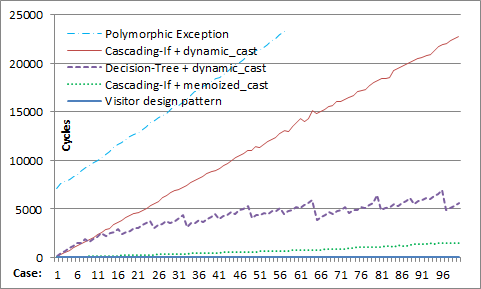
\includegraphics[width=0.47\textwidth]{DCast-vs-Visitors1.png}
  \caption{Type switching based on naive techniques}
  \label{fig:DCastVis1}
\end{figure}

When the class hierarchy is not flat and has several levels, the above 
cascading-if can be replaced with a decision tree that tests base classes first 
and thus eliminates many of the derived classes from consideration. This 
approach is used by Emir to deal with type patterns in Scala
\cite[\textsection 4.2]{EmirThesis}. The intent is to replace a sequence of 
independent dynamic casts between classes that are far from each other in the 
hierarchy with nested dynamic casts between classes that are close to each 
other. Another advantage is possibility to fail early: if the type of the subject 
does not match any of the clauses, we will not have to try all the cases. 
Flat hierarchy, which will likely be formed by the leafs in even a multi-level 
hierarchy, will not be able to benefit from this optimization and 
will effectively degrade to the above cascading-if. Nevertheless, when 
applicable, the optimization can be very useful and its benefits can be seen in
Figure~\ref{fig:DCastVis1} under ``Decision-Tree + dynamic\_cast''. The class 
hierarchy for this timing experiment was forming a perfect binary tree with 
classes number 2*N and 2*N+1 derived from a class with number N. The structure 
of the hierarchy also explains the repetitive pattern of timings.

The above solution either in a form of cascading-if or as a decision tree can be 
significantly improved by lowering the cost of a single \code{dynamic_cast}. 
We devise an asymptotically constant version of this operator that we call
\code{memoized_cast} in \textsection\ref{sec:memcast}. As can be seen from the graph 
titled ``Cascading-If + memoized\_cast'', it speeds up the above cascading-if 
solution by a factor of 18 on average, as well as outperforms the decision-tree 
based solution for a number of case clauses way beyond those that can happen in 
a reasonable program. We leave the discussion of the technique until 
\textsection\ref{sec:memcast}, while we keep it in the chart to give perspective on 
an even faster solution to dynamic casting. The slowest implementation in the 
chart based on exception handling facilities of C++ is discussed in 
\textsection\ref{sec:xpm}.

The approach of Gibbs and Stroustrup employs divisibility of numbers to obtain a 
tag allocation scheme capable of performing type testing in constant time. 
Extended with a mechanism for storing offsets required for this-pointer 
adjustments, the technique can be used for an extremely fast dynamic casting on 
quite large class hierarchies\cite{FastDynCast}. The idea is to allocate tags 
for each class in such a way that tag of a class D is divisible by a tag of a 
class B if and only if class D is derived from class B. For comparison purposes 
we handcrafted this technique on the above flat and binary-tree hierarchies and 
then redid the timing experiments from Figure~\ref{fig:DCastVis1} using the fast 
dynamic cast. The results are presented in Figure~\ref{fig:DCastVis2}. For 
reference purposes we retained ``Visitor Design Pattern'' and ``Cascading-If + 
memoized\_cast'' timings from Figure~\ref{fig:DCastVis1} unchanged. Note that 
the Y-axis has been scaled-up 140 times, which is why the slope of 
``Cascading-If + memoized\_cast'' timings is so much bigger.

\begin{figure}[htbp]
  \centering
    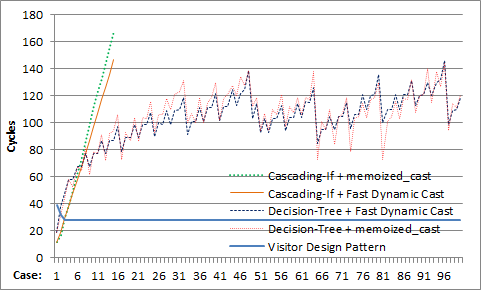
\includegraphics[width=0.47\textwidth]{DCast-vs-Visitors2.png}
  \caption{Type switching based on fast dynamic cast of Gibbs and Stroustrup\cite{FastDynCast}}
  \label{fig:DCastVis2}
\end{figure}

As can be seen from the figure the use of our memoized\_cast implementation can 
get close in terms of performance to the fast dynamic cast, especially 
when combined with decision trees. An important difference that cannot be seen 
from the chart, however, is that the performance of memoized\_cast is 
asymptotic, while the performance of fast dynamic cast is guaranteed. This 
happens because the implementation of memoized\_cast will incur an overhead of 
a regular dynamic\_cast call on every first call with a given most derived type. 
Once that class is memoized, the performance will remain as shown. Averaged over 
all calls with a given type we can only claim we are asymptotically as good as 
fast dynamic cast.

Unfortunately fast dynamic casting is not truly open to fully satisfy our 
checklist. The structure of tags required by the scheme limits the amount of 
classes it can handle. A 32-bit integer is estimated to be able to represent 7 
levels of a class hierarchy that forms a binary tree (255 classes), 6 levels of 
a similar ternary tree hierarchy (1093 classes) or just one level of a hierarchy 
with 9 base classes -- multiple inheritance is the worst case scenario of the 
scheme that quickly drains its allocation possibilities. Besides, similarly to 
other tag allocation schemes, presence of class extensions in DLLs will likely 
require an integration effort to make sure different DLLs are not reusing prime 
numbers in a way that might result in an incorrect dynamic cast.

Seeing predictably constant dispatching overhead of the visitor design pattern 
it became clear that any open solution that will have a non-constant dispatching 
overhead will have a poor chance of being adopted. Multi-way switch on 
sequentially allocated tags\cite{Spuler94} was one of the few techniques that 
could achieve constant overhead, and thus compete and even outperform visitors. 
Unfortunately the scheme has problems of its own that make it unsuitable.

%To better understand the problem let us look at some existing solutions to type 
%switching that we found to be used in practice. 

%From our experience on this project we have noticed that we can only compete 
%with visitors when switch statements are implemented with a jump table. As soon 
%as compiler was putting even a single branch into the decision tree of cases, 
%the performance was degraded significantly. From this perspective we do not 
%regard solutions based on decision trees as efficient, since they do not let us 
%compete compete with the visitors solution.

The simple scheme of assigning a unique tag per variant (instantiatable class 
here) will not pass our first question because the tags of base and derived 
classes will have to be different if the base class can be instantiated on its 
own. In other words we will not be able to land on a case label of a base class 
having a derived tag only. The already mentioned partitioning of tags of derived 
classes based on the classes in case clauses also will not help as it assumes 
knowledge of all the classes and thus fails extensibility through DLLs.

In practical implementations hand crafted for a specific class hierarchy, tags 
often are not chosen arbitrarily, but to reflect the subtyping relation of the 
underlain hierarchy. Switching on base classes in such setting will typically 
involve a call to some function $f$ that converts derived class' tag into a base 
class' tag. An example of such scheme would be having a certain bit in the tag 
set for all the classes derived from a given base class. Unfortunately this 
solution creates more problems than it solves.

First of all the solution will not be able to recognize an exceptional case 
where most of the derived classes should be handled as base class, while few 
should be handled specifically. Applying function $f$ puts several different 
types into an equivalence class with their base type, making them 
indistinguishable from each other.

Secondly, the assumed structure of tags is likely to make the set of tags 
sparse, effectively forcing compiler to use a decision tree instead of jump 
table to implement the switch. Even though conditional jump is reported to be 
faster than indirect jump on many computer architectures~\cite[\textsection 
4]{garrigue-98}, this did not seem to be the case in our experiments. Splitting 
of a jump table into two with a condition, that was sometimes happening because 
of our case label allocation scheme, was resulting in a noticeable degradation of 
performance in comparison to a single jump table.

Besides, as was seen on the scheme of Gibbs and Stroustrup, the assumed 
structure of tags can also significantly decrease the amount of classes a given 
allocation scheme can handle. It is also interesting to note that even though 
their scheme can be easily adopted for type switching with decision trees, it is 
not easily adoptable for type switching with jump tables: in order to obtain 
tags of base classes we will have to decompose the derived tag into primes and 
then find all the dividers of the tag, present in case clauses.

Summarizing, truly open and efficient type switching seems to be a non-trivial 
problem. The implementations we found in the literature where either open or 
efficient, but not both. Efficient implementation was typically achieved by 
sealing class hierarchy and using jump table. Without sealing, the implementation 
was resorting to decision trees and type testing, which was not efficient.
We are unaware of any efficient tag allocation scheme that can be used in a 
truly open scenario.

\section{Solution for Polymorphic Classes}
\label{sec:copc}

As mentioned, we approach type switching on polymorphic classes and tagged 
classes differently. In this subsection we outline the implementation of type 
switching on classes that have vtbl-pointer in their instances.

\subsection{Virtual Table Pointers}
\label{sec:vtp}

Before we discuss our solution we would like to talk about certain properties of 
the C++ run-time system that we rely on. Strictly speaking C++ standard does not 
require implementations to use any given technique (e.g. use virtual tables to 
implement virtual functions), however interoperability requirements have forced 
compiler vendors to design a set of rules called Application Binary Interface 
(ABI)\cite{C++ABI}. Most of the C++ compilers today follow these rules, with 
notable exception of Microsoft Visual C++. We show that the technique presented 
here will work with any C++ compiler that follows the C++ ABI. Microsoft's own 
ABI is not publically available and thus we could not verify that it satisfies 
our requirements. Nevertheless we did run numerous experiments with various 
class hierarchies and have sufficient confidence that our approach can be used 
in Visual C++. This is why we include experimental results for this compiler as 
well.

Besides single inheritance supported by most object-oriented languages, C++ 
supports multiple-inheritance of two kinds: repeated and virtual. Under repeated 
inheritance given derived class may inherit certain base class in several ways. 
Objects of such class will have several subobjects of that base class. Under 
virtual inheritance there will only be one shared subobject, accessible through 
different inheritance paths. Because of this peculiarity of the C++ type system 
it is not sufficient to talk only about static and dynamic types of an object -- 
one has to talk about a subobject of certain static type accessible through 
given inheritance path within a dynamic type.

The notion of subobject has been formalized before\cite{RF95,WNST06,RDL11}.
We follow here the presentation of Ramamanandro et al\cite{RDL11}.

A base class subobject of a given complete object is represented by a pair 
$\sigma = \langle h,l\rangle$ with $h \in \{Repeated,Shared\}$ representing the 
kind of inheritance (single inheritance is repeated with one base class) and $l$ 
representing the path in non-virtual inheritance graph.

A predicate $C\leftY\sigma\rightY A$ they introduce means that $\sigma$ 
designates a base class subobject of class $C$, with subobject's static type 
being $A$.

A class that declares or inherits a virtual function is called a 
\emph{polymorphic class}\cite[\textsection 10.3]{C++0x}. C++ ABI in turn defines 
\emph{dynamic class} to be a class requiring a virtual table pointer (because it 
or its bases have one or more virtual member functions or virtual base classes). 
A polymorphic class is thus a dynamic class by definition.

\emph{Virtual table pointer} (vtbl-pointer) is a member of object's layout 
pointing to a virtual table. \emph{Virtual table} is a table of information used 
to dispatch virtual functions, access virtual base class subobjects, and to 
access information for runtime type identification (RTTI). Because of repeated
inheritance an object of given type may have several vtbl-pointers in it. Each 
such pointer corresponds to one of the polymorphic base classes. Given an object 
$a$ of static type $A$ that has $k$ vtbl-pointers in it, we will use the same 
notion we use for regular fields to refer them: $a.vtbl_i$.

A \emph{primary base class} for a dynamic class is the unique base class (if any) 
with which it shares the virtual table pointer at offset 0. The data layout 
procedure for non-POD types described in \textsection2.4 of C++ ABI 
requires dynamic classes either to allocate vtable pointer at offset 0 or share 
the virtual table pointer from its primary base class, which is by definition at 
offset 0. For our purpose this means that we can rely on virtual table pointer 
always be present at offset 0 for all dynamic classes, and thus all polymorphic 
classes.

\begin{lemma}
In an object layout that adheres to C++ ABI, a polymorphic class always has a 
virtual table pointer at offset 0.
\label{lem:vtbl}
\end{lemma}

%C++ standard requires an argument of \code{dynamic_cast} to be a pointer to or 
%an lvalue of a polymorphic type when performing \emph{downcast} -- a cast from 
%base to derived\cite[\textsection 5.2.7-6]{C++0x}. We can thus always safely 
%extract virtual table pointer from offset 0 of any valid argument to 
%\code{dynamic_cast}.

%Similarly, each class that has virtual member functions or virtual bases has an 
%associated set of virtual tables. There may be multiple virtual tables for a 
%particular class, if it is used as a base class for other classes. However, the 
%virtual table pointers within all the objects (instances) of a particular 
%most-derived class point to the same set of virtual tables.

\noindent
The exact content of the virtual table is not important for this discussion. We 
would like to point out a few fields in it that we will refer to later.

\begin{itemize}
\setlength{\itemsep}{0pt}
\setlength{\parskip}{0pt}
\item The \emph{typeinfo pointer} points to the typeinfo object used for RTTI. 
      It is always present.  
\item The \emph{offset to top} holds the displacement to the top of the object 
      from the location within the object of the virtual table pointer that 
      addresses this virtual table, as a \code{ptrdiff_t}. It is always present.
\item \emph{Virtual Base (vbase) offsets} are used to access the virtual bases 
      of an object. Such an entry is added to the derived class object address 
      (i.e. the address of its virtual table pointer) to get the address of a 
      virtual base class subobject. Such an entry is required for each virtual 
      base class.
\end{itemize}

\noindent
Given a virtual table pointer \code{vtbl}, we will refer to these fields as 
\code{rtti(vtbl)}, \code{off2top(vtbl)} and \code{vbase(vtbl)} respectively. 
We will also assume presence of function $offset(\sigma)$ that defines the 
offset of the base class identified by the end of the path $\sigma$ within a 
class identified by its first element.

\begin{theorem}
In an object layout that adheres to C++ ABI, if virtual table pointers of two 
objects of the same static type are the same, then they both refer to subobjects 
with the same inheritance path in the same most-derived type.
\begin{eqnarray*}
    \forall a_1, a_2 : A\ |\ a_1\in C_1\leftY\sigma_1\rightY A \wedge a_2\in C_2\leftY\sigma_2\rightY A \\
    a_1.vtbl_i = a_2.vtbl_i \Rightarrow C_1 = C_2 \wedge \sigma_1 = \sigma_2
\end{eqnarray*}
\label{thm:vtbl}
\end{theorem}
\begin{proof}
Let us assume first $a_1.vtbl_i = a_2.vtbl_i$ but $C_1 \neq C_2$. In this case we 
have \code{rtti}$(a_1.vtbl_i) = $\code{rtti}$(a_2.vtbl_i)$. By definition 
\code{rtti}$(a_1.vtbl_i) = C_1$ while \code{rtti}$(a_2.vtbl_i) = C_2$, which 
contradicts that $C_1 \neq C_2$. Thus $C_1 = C_2 = C$.

Let us assume now that $a_1.vtbl_i = a_2.vtbl_i$ but $\sigma_1 \neq \sigma_2$. 
Let $\sigma_i=\langle h_i,l_i\rangle,i=1,2$ 

If $h_1 \neq h_2$ then one of them refers to virtual base while the other to 
repeated. Assuming $h_1$ refers to virtual path, \code{vbase}$(a_1.vtbl_i)$ has 
to be defined inside the vtable accordingly to ABI, while 
\code{vbase}$(a_2.vtbl_i)$ -- should not. This would contradict again that both 
$vtbl_i$ refer the same virtual table.

We have thus $h_1 = h_2 = h$. If $h = Shared$ than there is only one path to 
such $A$ in $C$, which would contradict $\sigma_1 \neq \sigma_2$. 
If $h = Repeated$ then we must have that $l_1 \neq l_2$. In this case let $k$ be 
the first position in which they differ: 
$l_1^j=l_2^j \forall j<k \wedge l_1^k\neq l_2^k$. Since our class $A$ is a base 
class for classes $l_1^k$ and $l_2^k$, both of which are in turn base classes of 
$C$, object identity requirement of C++ require that the relevant subobjects of 
type $A$ have different offsets within class $C$: 
$offset(\sigma_1)\neq offset(\sigma_2)$ However 
$offset(\sigma_1)=$\code{off2top}$(a_1.vtbl_i)=$\code{off2top}$(a_2.vtbl_i)=offset(\sigma_2)$ 
since $a_1.vtbl_i = a_2.vtbl_i$, which contradicts that offsets are different.
\end{proof}

Conjecture in the other direction is not true in general as there may be 
duplicate virtual tables for the same type present at run-time. This happens in 
many C++ implementations in the presence of dynamically linked libraries as the
same class compiled into executable and into DLL it loads may have compiler 
allocate identical virtual tables inside executable's and DLL's binaries.

\begin{corollary}
Results of \code{dynamic_cast} can be reapplied to a different instance from 
within the same subobject. 

$\forall A,B \forall a_1, a_2 : A\ |\ a_1.vtbl_i = a_2.vtbl_i \Rightarrow$ \\
\code{dynamic_cast<B>}$(a_1).vtbl_j = $\code{dynamic_cast<B>}$(a_2).vtbl_j \vee$ \\
\code{dynamic_cast<B>}$(a_1)$ throws $\wedge$ \code{dynamic_cast<B>}$(a_2)$ throws.
\label{crl:vtbl}
\end{corollary}

Lastly we would like to point out that during construction and deconstruction of 
an object, a value of a given virtual table pointer may change. In particular 
that value will reflect the dynamic type of the object to be the type of the 
fully constructed part only. This fact does not affect our reasoning, as during 
such transition we also treat the object to have the type of its fully 
constructed base only. Such interpretation is in line with the C++ semantics for 
virtual function calls and use of RTTI during construction and destruction of an 
object. Once the complete object is fully constructed, the value of the virtual 
table pointer will remain the same for the lifetime of the object.

\subsection{Memoization Device}
\label{sec:memdev}

Let us look at a slightly more general problem than type switching. Consider a 
generalization of switch statement that takes predicates on a subject as its 
clauses and executes the first statement $s_i$ whose predicate got enabled: 

\begin{lstlisting}
switch (x)
{
case P1(x): s1;
 ...
case Pn(x): sn;
}
\end{lstlisting}

\noindent
Assuming that predicates depend only on $x$ and nothing else as well as that 
they do not involve any side effects, we can be sure that the next time we come 
to such switch with the same value, the same predicate will become enabled 
first. Thus, we would like to avoid evaluating predicates and jump straight to 
the statement it guards. In a way we would like the switch to  memoize which 
case becomes enabled for a given value of $x$.

Inspired by Duff's Device\cite{Duff} we devised a construct that we call 
\emph{Memoization Device} that does just that:

\begin{lstlisting}
typedef decltype(x) T;
static std::unordered_map<T,int> jump_target_map;

switch (int& target = jump_target_map[x])
{
default: // entered when we haven't seen x yet
    if (P1(x)) { target = 1;   case 1: s1; } else 
    if (P2(x)) { target = 2;   case 2: s2; } else
      ...
    if (Pn(x)) { target = n;   case n: sn; } else
                 target = n+1;
case n+1: // none of predicates is true on x
}
\end{lstlisting}

\noindent
The static \code{jump_target_map} maps values to jump targets, and will be 
allocated upon first entry to the function. The map is initially empty and is 
updated from within the switch as we proceed through the interleaved 
cascading-if statement. Accordingly to the logic of STL's \code{unordered_map}, 
a key $x$ that is not yet in the map will result in allocation of a new entry 
with its associated data (of type int) default initialized to 0. Since there is 
no case label 0 in the switch, default case will be taken, which, in turn, will 
initiate sequential execution of the interleaved cascading-if statement.

The sequential execution of the cascading-if statement will keep checking 
predicates $P_j(x)$ until the first predicate $P_i(x)$ that returns true. By 
assigning $i$ to \code{target} we will effectively associate $i$ with $x$ since 
\code{target} is just a reference to \code{jump_target_map[x]}. This association 
will make sure that the next time we are called with the value $x$ we will jump 
directly to the label $i$. When none of the predicates returns true, we will 
record it by associating $x$ with $n+1$, so that the next time we can jump 
directly to the end of the switch on $x$. 

The above construct effectively gives the entire statement first-fit semantics. 
In order to evaluate all the statements, whose predicates are true, and thus 
give the construct all-fit semantics, we might want to be able to preserve the 
fall-through behavior of the switch. In this case we can still skip the initial 
predicates returning false and start from the first successful one. This can be 
easily achieved by removing all else statements and making if-statements 
independent as well as wrapping all assignments to \code{target} with condition, 
to make sure only the first successful predicate executes it:

\begin{lstlisting}
    if (Pi(x)) { if (target == 0) target = i; case i: si; }
\end{lstlisting}

\noindent
Note that the protocol that has to be maintained by this structure does not 
depend on the actual value of case labels. The only property we rely on here is 
that they are all different and that there is a predefined default value, 
distinct from any of them. In fact, the default clause we used here can be 
replaced with case clause with the predefined value. From experience, however, 
we have noticed that keeping the default clause results in a faster code. A more 
important performance consideration is to keep the values close to each other. 
Not following this rule might result in compiler choosing decision tree over a 
jump table implementation of the switch, which will significantly degrade the 
performance.

The first-fit semantics is not an inherent property of memoization device however. 
Assuming that conditions are either mutually exclusive or imply one another we 
can build a decision-tree based memoization device that will effectively have 
\emph{most specific} semantics -- an analog of best-fit semantics in predicate 
dispatching\cite{ErnstKC98}.

Imagine that predicates with numbers $2i$ and $2i+1$ are mutually exclusive and 
each imply the value of the predicate with number $i$ i.e. $\forall x \in Domain(P)$
\begin{eqnarray*}
P_{2i+1}(x)\rightarrow P_i(x) \wedge P_{2i}(x)\rightarrow P_i(x) \wedge \neg(P_{2i+1}(x) \wedge P_{2i}(x))
\end{eqnarray*}
\noindent
The following decision-tree based memoization device will execute the statement 
$s_i$ associated with the \emph{most specific} (i.e. the predicate that implies 
all other predicates true on $x$) predicate $P_i$ that evaluates to true or will 
skip the entire statement if none of the predicates is true on $x$.

\begin{lstlisting}
switch (int& target = jump_target_map[x])
{
default:
    if (P1(x)) {
        if (P2(x)) {
            if (P4(x)) { target = 4; case 4: s4; } else
            if (P5(x)) { target = 5; case 5: s5; } 
            target = 2; case 2: s2;
        } else
        if (P3(x)) {
            if (P6(x)) { target = 6; case 6: s6; } else
            if (P7(x)) { target = 7; case 7: s7; } 
            target = 3; case 3: s3;
        }
        target = 1; case 1: s1;
    } else {
        target = 0; case 0:   ;
    }
}
\end{lstlisting}

\noindent
An example of predicates that satisfy this condition are class membership tests
where the truth of a predicate that tests membership in a derived class implies 
the truth of a predicate that tests membership in its base class. Our library 
solution prefers the simpler cascading-if approach only because the necessary 
structure of the code can be laid out directly with macros. A compiler solution 
will use the decision-tree approach whenever possible to lower the cost of the 
first match from linear in case's number to logarithmic as seen in Figure\ref{fig:DCastVis1}.

When the predicates do not satisfy the implication or mutual exclusion property 
mentioned above, a compiler of a language based on predicate dispatching would 
typically issue an ambiguity error. Some languages might choose to resolve it 
accordingly to lexical or some other ordering. In any case, presence of 
ambiguities or their resolution has nothing to do with memoization device 
itself. The latter only helps optimize the execution once a particular choice of 
semantics has been made and code implementing it has been laid out.

The main advantage of memoization device is that it does not impose any 
restriction on the type of a subject. It can easily support multiple scrutiny 
by turning $x$ into a tuple. Another advantage is that conditions and statements 
do not have to be repeated several times textually, which lets us turn the 
boilerplate code of maintaining memoization logic into macros.

The main disadvantage of such solution is of course the size of the hash table 
that grows proportionally to the amount of different values coming through the 
function. We will see, however, that often times the values can be grouped into 
equivalence classes, such that values in the same class do not change the 
predicate. The map can then associate an equivalence class of a value with 
target instead of associating value with it.

\subsection{V-Table Pointer Memoization}
\label{sec:vtblmem}

Memoization device can almost immediately be used for multi-way type testing by 
using \code{dynamic_cast<Di>} as a predicate $P_i$. This cannot be considered a 
type switching solution, however, as one would expect to also have a reference 
to the uncovered type. Using a \code{static_cast<Di>} upon successful type test 
would have been a solution if we did not have multiple inheritance. It is 
certainly can be used as such in languages with only single inheritance, e.g. 
Java. For the fully functional C++ solution, we combine memoization device with 
the properties of virtual table pointers into a \emph{V-Table Pointer 
Memoization} technique.

We showed in Corollary~\ref{crl:vtbl} that the results of dynamic cast can be 
reapplied on subobjects with the same virtual table pointer. With this in mind, 
we can now apply memoization device to polymorphic objects grouped by their 
vtbl-pointer. The head of the switch requires few extra definitions:

\begin{lstlisting}
typedef std::pair<ptrdiff_t,size_t> type_switch_info;
static std::unordered_map<intptr_t, type_switch_info> jump_target_map;
intptr_t          vtbl = *reinterpret_cast<const intptr_t*>(p);
type_switch_info& info = jump_target_map[vtbl];
const void*       tptr; 
\end{lstlisting}

\noindent
We use the virtual table pointer extracted from a polymorphic object pointed to 
by \code{p} as a key for association. The value stored along the key in 
association now keeps both: the target for the switch as well as a memoized 
offset for dynamic cast. The snippet corresponding to the $i^{th}$ case now 
looks as following:

\begin{lstlisting}
    if (tptr = dynamic_cast<const Di*>(p)) {
        if (info.second == 0) {
            info.first  = intptr_t(tptr)-intptr_t(p); // offset
            info.second = @$i$@; // jump target
        }
case @$i$@: // @$i$@ is a constant here - clause's position in switch
        auto matched = adjust_ptr<Di>(p,info.first); 
        si;
    }
\end{lstlisting}

\noindent
The main condition remains the same. We keep check for the first initialization 
because we allow the fall-through semantics here, letting user break from the 
switch when needed. Upon first entry we compute the offset that the dynamic cast 
performed and save it together with target associated to the virtual table 
pointer. On the next iteration we will jump directly to the case label and 
restore the invariant of \code{matched} being a properly casted reference to the 
derived object.

The use of dynamic cast makes a huge difference in comparison to the use of 
static cast we dismissed above. First of all the C++ type system is much more 
restrictive about static cast and many cases where it is not allowed can 
still be handled by dynamic cast. Examples of these include downcasting from an 
ambiguous base class or cross-casting between unrelated base classes.

An important benefit we get from this optimization is that we do not store the 
actual values (pointers to objects) in the hash table anymore, but group them 
into equivalence classes based on their virtual table pointers. The amount of 
such pointers in a program is always bound by $O(|A|)$, where $A$ represents the 
static type of an object, while $|A|$ represents the amount of classes directly 
or indirectly derived from $A$. The linear coefficient hidden in big-o notation 
reflects possibly multiple vtbl-pointers in derived classes due to the use of 
multiple inheritance.

However, most important benefit of this optimization is the constant time on average 
used to dispatch each of the case clauses, regardless of their position in the 
type switch. The constant time on average is coming from the average complexity 
of accessing an element in \code{unordered_map}, while its worst complexity can 
be proportional to the size of the map. We show in the next section, however, 
that most of the time we will be bypassing traditional access to elements of the 
map, cause as is, the type switch is still about 50\% slower than the visitor 
design pattern.

%Note that we can apply the reasoning of \textsection\ref{sec:memdev} and change 
%the first-fit semantics of the resulting match statement into a best-fit 
%semantics simply by changing the underlain cascading-if structure with decision 
%tree. A compiler implementation of a type switch based on V-Table Pointer 
%Memoization will certainly take advantage of this optimization to cut down the 
%cost of the first run on a given vtbl-pointer, when the actual memoization happens.

\subsubsection{Structure of Virtual Table Pointers}
\label{sec:sovtp}

In our numerous experiments with several compilers and different class 
hierarchies we noticed that virtual table pointers were not entirely random 
addresses in memory and had certain structure. Virtual tables of classes related 
by inheritance were grouped together in memory most of the time, making the 
values of vtbl-pointers pointing to them follow a certain pattern. For example, 
a set of 100 virtual table pointers that came through a type switch in one of 
our test programs were all of the form 
\texttt{00000001001111100000X11XXXXXXX00}, where X indicates positions in which 
bits in at least two address were different.

Virtual table pointers are not constant values and are not even guaranteed to be 
the same between different runs of the same application. Techniques like 
\emph{address space layout randomization} or simple \emph{rebasing} of the entire 
module are likely to change these values. The relative distance between them is 
likely to remain the same though as long as they come from the same module.

The common bits on the right come from the virtual table size and alignment 
requirements and depending on compiler, configuration and class hierarchy could 
easily vary from 2 to 6 bits. Because the vtbl-pointer under C++ ABI points into 
an array of function pointers, the alignment requirement of 4 bytes for those 
pointers on a 32-bit architecture is what makes at least the last 2 bits to be 0. 
For our purpose the exact amount of bits on the right is not important as we 
evaluate this amount at run time based on vtbl-pointers seen so far. Here we only 
would like to point out that there would be some amount of common bits on the 
right.

Another observation we made during our experiments with vtbl-pointers of various 
existing applications was that the values of the pointers where changing more 
frequently in the lower bits than in the higher ones. We believe that this was 
happening because programmers tend to group multiple derived classes in the same 
translation unit so the compiler was emitting virtual tables for them close to 
each other as well. 

Note that derived classes that do not introduce their own virtual functions 
(even if they override some existing ones) are likely to have virtual tables of 
the same size as their base class. Even when they do add new virtual functions 
the size of their virtual tables can only increase in comparison to their base 
classes. This is why the difference between many consecutive vtbl-pointers that 
came through a given match statement was usually constant or very slightly 
different.

The changes in higher bits were typically due to separate compilation and 
especially due to dynamically loaded modules. When a DLL is loaded it may have 
its own copy of v-tables for classes also used in other modules as well as 
v-tables for classes it introduces. Comparing all vtbl-pointers coming only from 
that DLL we can get a different pattern \texttt{01110011100000010111XXXXXXXXX000} 
and when compared over all the loaded modules the pattern will likely become 
something like \texttt{0XXX00X1X0XXXXXX0XXXXXXXXXXXXX00}. Overall they were not 
changing the general tendency we saw: smaller bits were changing more frequently 
than larger ones with the exception of lowest common bits of course.

These observations made virtual table pointers of classes related by inheritance 
ideally suitable for indexing -- the values obtained by throwing away the common 
bits on the right were compactly distributed in small disjoint ranges. We use 
those values to address a cache built on top of the hash table in order to 
eliminate a hash table lookup in most of the cases.  The important 
guarantee about the validity of the cached hash table references comes from the 
C++0x standard, which states that ``insert and emplace members shall not affect 
the validity of references to container elements''\cite[\textsection 
23.2.5(13)]{C++0x}. 

Depending on the amount of actual collisions that happen in the cache, our 
v-table pointer memoization technique can come close and even outperform the 
visitor design pattern. The numbers are, of course, averaged over many runs as 
the first run on every most derived type will take time shown in 
Figure\ref{fig:DCastVis1}. We did however test our technique on real code and 
can confirm that it does perform well in the real-world use cases.

The information about jump targets and necessary offsets is just an example of 
information we might want to be able to associate with and access via virtual 
table pointers. Our implementation of \code{memoized_cast} from 
\textsection\ref{sec:memcast} effectively reuses this general data structure with 
a different type of element values. We thus created a generic reusable class 
\code{vtblmap<T>} that maps vtbl-pointers to elements of type T. We will refer 
to the combined cache and hash-table data structure extended with the logic for 
minimizing conflicts presented below as \emph{vtblmap} data structure.

\subsubsection{Minimization of Conflicts}
\label{sec:moc}

The small amount of cycles that the visitor design pattern needs to uncover a 
type does not let us put too sophisticated cache indexing mechanisms into the 
critical path of execution. This is why we limit our indexing function to shifts 
and masking operations as well as choose the size of cache to be a power of 2.

As usual, by \emph{conflict} we mean a situation in which two or more virtual 
table pointers are mapped to the same location in cache using given indexing 
function. Presence of conflicts means that accessing values of \code{vtblmap<T>} 
associated with some vtbl-pointers may result in a slower lookup of the element 
inside the underlying hash table as opposed to direct fetch from the cache.
This `slower' lookup, as we mentioned, is constant on average and linear in the 
size of the hash map in the worst case.

Given $n$ vtbl-pointers we can always find a cache size that will render no 
conflicts between them. The necessary size of such cache, however, can be too 
big to justify the use of memory. This is why in our current implementation we 
always consider only 2 different cache sizes: $2^k$ and $2^{k+1}$ where $2^{k-1} 
\le n \leq 2^k$. This guarantees us that the cache size is never more than 4 
times bigger than the minimum required cache size.

During our experiments we noticed that often times the change in the smallest 
different bit happens only in very few vtbl-pointers, which effectively was 
cutting the available cache space in half. To overcome this problem we let the 
amount of bits we shift the vtbl-pointer by vary further and compute it in such 
a way that minimizes the number of conflicts.

To avoid doing any computations in the critical path \code{vtblmap} only 
recomputes the optimal shift and the size of the cache when an actual collision 
happens. In order to avoid constant recomputations when conflicts are unavoidable, 
we add an additional restriction of only reconfiguring the optimal parameters if 
the amount of vtbl-pointers in the \code{vtblmap} has increased since the last 
recomputation. Since the amount of vtbl-pointers is of the order $O(|A|)$, where 
$A$ is the static type of all vtbl-pointers coming through a \code{vtblmap}, the 
restriction assures that reconfigurations will not happen infinitely often.

To minimize the amount of recomputations even further, our library communicates 
to the \code{vtblmap<T>} through its constructor the amount of case clauses in 
the underlain match statement. We use this number as an estimate of expected 
size of \code{vtblmap} and pre-allocate the cache accordingly to this estimated 
number. The cache is still allowed to grow based on the actual amount of 
vtbl-pointers that comes through a \code{vtblmap}, but it never shrinks from the
initial value. This improvement significantly minimizes the amount of collisions 
at early stages as well as the number of possibilities we have to consider 
during reconfiguration.

The above logic of \code{vtblmap} always chooses the configuration that renders 
no conflicts, when such a configuration is possible during recomputation of 
optimal parameters. When this is not possible it is natural to prefer collisions 
to happen on less frequent vtbl-pointers.

We studied frequency of vtbl-pointers that come through various match statements
of a C++ pretty-printer that we implemented on top of the Pivot 
framework\cite{Pivot09} using our pattern-matching library. We ran the pretty 
printer through a set of C++ standard library headers and then ranked all the 
classes from the most frequent to the least frequent ones on average. The 
resulting probability distribution, resembled power-law distribution, which meant 
that for that specific application probability of some vtbl-pointers was much 
higher than the probability of many other vtbl-pointers taken altogether. In 
our case the 2 most frequent classes were representing the use of a variable in 
a program, and their combined frequency was larger than the frequency of all the 
other nodes. Naturally we would like to avoid conflicts on such classes in the 
cache when possible.

To do this, our library provides a configuration flag that enables tracing 
frequencies of each vtbl-pointer in a switch and then uses this information to 
minimize the amount of conflicts. Due to page limitations, we refer the reader 
to the technical report accompanying this paper for more details on our 
experiments with the use of vtbl-pointer frequencies\cite{TR}. Here we will only 
mention that by default we do not enable frequency tracing because the 
significant drop in the amount of actual collisions was not reflected in a 
noticeable decrease in execution time. This was happening because the total 
amount of actual collisions even in non-frequency based caching was much smaller 
than the amount successful cache hits.

\section{Solution for Tagged Classes}
\label{sec:cotc}

Memoization device outlined in \textsection\ref{sec:memdev} can in principle be 
applied to tagged classes too. The dynamic cast will be replaced by a small 
compile-time template meta-program that checks whether class associated with 
given tag is derived from the target type of the case clause. If so, the static 
cast can be used to obtain the offset.

Despite its straightforwardness we felt that it should be possible to do better 
than the general solution, given that each class is already identified with a 
dedicated constant known at compile time.

As we mentioned in \textsection\ref{sec:poets}, nominal subtyping of C++ 
effectively gives every class multiple types. The idea is thus to associate with 
the type not only its most derived tag, but also the tags of all its base classes.
In a compiler implementation such a list can be stored inside the virtual table 
of a class, while in our library solution it is shared between all the instances 
with the same most derived tag in a less efficient global map, associating the 
tag to its tag list.

The list of tags is topologically sorted accordingly to the subtyping relation 
and terminates with a dedicated value distinct from all the tags. We call such a 
list a \emph{Tag Precedence List} (TPL) as it resembles the \emph{Class 
Precedence List} (CPL) of object-oriented descendants of Lisp (e.g. Dylan, 
Flavors, LOOPS, and CLOS) used there for \emph{linearization} of class 
hierarchies. The classes in CPL are ordered from most specific to least specific 
with siblings listed in the \emph{local precedence order} -- the order of the 
direct base classes used in the class definition. TPL is just an implementation 
detail and the only reason we distinguish TPL from CPL is that in C++ classes 
are often separated into interface and implementation classes and it might so 
happen that the same tag is associated by the user with an interface and several 
implementation classes. 

A type switch below, built on top of a hierarchy of tagged classes, proceeds as 
regular switch on the subject's tag. If the jump succeeds, we found an exact 
match, otherwise we get into a default clause that obtains the next tag in the 
tag precedence list and jump back to the beginning of the switch statement for a 
rematch:

\begin{lstlisting}
    const size_t* taglist = 0;
          size_t  attempt = 0;
          size_t  tag     = object->tag;
ReMatch:
    switch (tag) 
    {
    default:
        if (!taglist) 
            taglist = get_taglist(object->tag);
        tag = taglist[++attempt];
        goto ReMatch;
    case end_of_list: break;
    case bindings<D1>::kind_value: s1; break;
    ...
    case bindings<Dn>::kind_value: sn; break;
    }
\end{lstlisting}

\noindent
The above structure lets us dispatch to case clauses of the most derived class 
with an overhead of initializing two local variables compared to a switch on a 
sealed hierarchy. Dispatching to a case clause of a base class will take a time 
roughly proportional to the distance between the matched base class and the most 
derived class in the inheritance graph. When none of the base class tags was 
matched we will necessarily reach the end\_of\_list marker in the tag precedence 
list and thus exit the loop.

Our library automatically builds the function \code{get_taglist} based on 
additional definitions that user provides inside \code{bindings}. The details 
can be found in our accompanying paper\cite{AP}.

\section{(Ab)using Exceptions for Type Switching}
\label{sec:xpm}

Several authors had noted the relationship between exception handling and type 
switching before\cite{Glew99,ML2000}. Not surprisingly, the exception handling 
mechanism of C++ can be abused to implement the first-fit semantics of a type 
switch statement. The idea is to harness the fact that catch-handlers in C++ 
essentially use first-fit semantics to decide which one is going to handle a 
given exception. The only problem is to raise an exception with a static type 
equal to the dynamic type of the subject.

To do this, we employ \emph{polymorphic exception} idiom\cite{PolyExcept} that 
introduces a virtual function \code{virtual void raise() const = 0;} into the 
base class, overridden by each derived class in syntactically same way: 
\code{throw *this;}. Match statement then simply calls \code{raise} on subject, 
while case clauses are turned into catch-handlers. The exact name of the 
function is not important and is communicated to the library via 
\code{bindings}. The \code{raise} member function can be seen as an analog of 
\code{accept} member function in visitor design pattern, whose main purpose is 
to discover subject's most specific type. The analog of a call to \code{visit} 
to communicate that type is replaced in this scheme with exception unwinding 
mechanism.

Just because we can, it does not mean we should abuse the exception handling 
mechanism to give us the desired control flow. In the table-driven approach 
commonly used in high-performance implementations of exception handling, the 
speed of handling an exception is sacrificed to provide a zero execution-time 
overhead for when exceptions are not thrown\cite{Schilling98}. Using exception 
handling to implement type switching will reverse the common and exceptional 
cases, significantly degrading performance. As can be seen in 
Figure\ref{fig:DCastVis1}, matching the type of the first case clause with 
polymorphic exception approach takes more than 7000 cycles and then grows 
linearly (with the position of case clause in the match statement), making it the 
slowest approach. The numbers illustrate why exception handling should only be 
used to deal with exceptional and not common cases.

Despite its total impracticality, the approach gave us a very practical idea of 
harnessing a C++ compiler to do \emph{redundancy checking} at compile time.

\subsection{Redundancy Checking}
\label{sec:redun}

Redundancy checking is only applicable to first-fit semantics of the match 
statement, and warns the user of any case clause that will never be entered 
because of preceding one being more general.

We provide a library-configuration flag, which, when defined, effectively turns 
the entire match statement into a try-catch block with handlers accepting the 
target types of the case clauses. This forces the compiler to give warning when 
more general catch handler preceds more specific one effectively performing a 
redundancy checking for us, e.g.:

\begin{lstlisting}
filename.cpp(55): warning C4286: 'ipr::Decl*' : is caught by 
                  base class ('ipr::Stmt*') on line 42
\end{lstlisting}

\noindent
Note that message contains both: a line number of the redundant case clause (55) 
and the line number of the case clause it is made redundant with (42).

Unfortunately the flag cannot be always enabled as case labels of the underlying 
switch statement have to be eliminated in order to render a syntactically 
correct program. Nevertheless, we found the redundancy checking facility of the 
library extremely useful when rewriting visitors based code: even though the 
order of overrides in visitor's implementation does not matter, for some reason 
more general ones were inclined to happen before specific ones in the code we 
looked at. Perhaps we are inclined to follow the class declaration order when 
defining and implementing visitors.

A related \emph{completeness checking} -- test of whether a given match 
statement covers all possible cases -- needs to be reconsidered for extensible 
data types like classes, since one can always add new variant to it. 
Completeness checking in this case may simply become equivalent to ensuring that 
there is either a default clause in the type switch or a clause with static type 
of a subject as a target type. In fact, our library has an analog of default 
clause called \code{Otherwise}-clause, which is implemented under the hood 
exactly as a regular case clause with subject's static type as a target type.

\section{Memoized Dynamic Cast}
\label{sec:memcast}

We saw in Corollary~\ref{crl:vtbl} that the results of \code{dynamic_cast} can 
be reapplied to a different instance from within the same subobject. This leads 
to a simple idea of memoizing the results of \code{dynamic_cast} and then using 
them on subsequent casts. In what follows we will only be dealing with the  
pointer version of the operator since the version on references that has a 
slight semantic difference can be easily implemented in terms of the pointer one.

The \code{dynamic_cast} operator in C++ involves two arguments: a value argument 
representing an object of a known static type as well as a type argument 
denoting the runtime type we are querying. Its behavior is twofold: on one side 
it should be able to determine when the object's most derived type is not a 
subtype of the queried type (or when the cast is ambiguous), while on the other 
it should be able to produce an offset to adjust the value argument by when it is.

We mimic the syntax of \code{dynamic_cast} by defining:

\begin{lstlisting}
template <typename T, typename S>
inline T memoized_cast(S* p);
\end{lstlisting}

\noindent
which lets the user replace all the uses of \code{dynamic_cast} in the program 
with \code{memoized_cast} with a simple:

\begin{lstlisting}
#define dynamic_cast memoized_cast
\end{lstlisting}

\noindent
It is important to stress that the offset is not a function of source and target 
types of \code{dynamic_cast} operator, which is why we cannot simply memoize the 
outcome inside the individual instantiations of \code{memoized_cast}.
The use of repeated multiple inheritance will result in classes having several 
different offsets associated with the same pair of source and target types 
depending on which subobject the cast is performed from. Accordingly to 
corollary~\ref{crl:vtbl}, however, it is a function of target type and the value 
of the vtbl-pointer stored in the object, because the vtbl-pointer uniquely 
determines the subobject within the most derived type. Our memoization of 
results of \code{dynamic_cast} should thus be specific to a vtbl-pointer and the 
target type. 

Our actual solution uses separate indexing of target types per each source type 
they are used with as well as allocates a different 
\code{vtblmap<std::vector<std::ptrdiff_t>>} for every source type. This lets us 
minimize unused entries within offset vectors by making sure only the plausible 
target types for a given source type are indexed. This solution should be 
suitable for most of the applications since we expect to have a fairly small 
amount of source types of \code{dynamic_cast} operator with a much larger amount 
of target types. For the unlikely case of small amount of target types and large 
amount of source types we let the user to revert the default behavior with a 
library configuration switch that allocates a single \code{vtblmap} per target type.

Use of \code{memoized_cast} to implement match statement potentially reuses the 
results of \code{dynamic_cast} computation across multiple independent match 
statements. This allows leveraging the cost of expensive first call with a 
given vtbl-pointer even further across all the match statements inside the 
program. The above define, with which a user can easily turn all dynamic casts 
into memoized casts can be used to speed-up existing code that uses dynamic 
casting without any refactoring overhead.

\section{Evaluation} %%%%%%%%%%%%%%%%%%%%%%%%%%%%%%%%%%%%%%%%%%%%%%%%%%%%%%%%%%%
\label{sec:eval}

\begin{figure*}
\begin{tabular}{@{}c@{ }l||@{ }r@{}@{ }r@{}|@{ }r@{}@{ }r@{}||@{ }r@{}@{ }r@{}|@{ }r@{}@{ }r@{}||@{ }r@{}@{ }r@{}|@{ }r@{}@{ }r@{}}
\hline % -----------------------------------------------------------------------------------------------------------------------------------------
\hline % -----------------------------------------------------------------------------------------------------------------------------------------
 &            & \multicolumn{4}{c||}{G++/32}  & \multicolumn{4}{c||}{MS Visual C++/32} & \multicolumn{4}{c}{MS Visual C++/64} \\
\hline % -----------------------------------------------------------------------------------------------------------------------------------------
 & Syntax     & \multicolumn{2}{c|}{Unified} & \multicolumn{2}{c||}{Special} & \multicolumn{2}{c|}{Unified} & \multicolumn{2}{c||}{Special} & \multicolumn{2}{c|}{Unified} & \multicolumn{2}{c}{Special} \\
\hline % -----------------------------------------------------------------------------------------------------------------------------------------
 & Encoding   & \Opn  & \Cls  & \Opn  & \Cls  & \Opn  & \Cls  & \Opn  & \Cls  & \Opn  & \Cls  & \Opn  & \Cls   \\
\hline % -------------------------------------------------------------------------------------------------
\hline % -------------------------------------------------------------------------------------------------
 & Repetitive &\gwNGPp&\gwNGKp&\gwNSPp&\gwNSKp&\VwNGPp&\VwNGKp&\VwNSPp&\VwNSKp&\VxNGPp&\VxNGKp&\VxNSPp&\VxNSKp \\
 & Sequential &\gwNGPq&\gwNGKq&\gwNSPq&\gwNSKq&\VwNGPq&\VwNGKq&\VwNSPq&\VwNSKq&\VxNGPq&\VxNGKq&\VxNSPq&\VxNSKq \\
 & Random     &\gwNGPn&\gwNGKn&\gwNSPn&\gwNSKn&\VwNGPn&\VwNGKn&\VwNSPn&\VwNSKn&\VxNGPn&\VxNGKn&\VxNSPn&\VxNSKn \\
\hline % --------------------------------------------------------------------------------------------------
\multirow{3}{*}{\begin{sideways}{\tiny Forward}\end{sideways}}
 & Repetitive &\gwYGPp&\gwYGKp&\gwYSPp&\gwYSKp&\VwYGPp&\VwYGKp&\VwYSPp&\VwYSKp&\VxYGPp&\VxYGKp&\VxYSPp&\VxYSKp \\
 & Sequential &\gwYGPq&\gwYGKq&\gwYSPq&\gwYSKq&\VwYGPq&\VwYGKq&\VwYSPq&\VwYSKq&\VxYGPq&\VxYGKq&\VxYSPq&\VxYSKq \\
 & Random     &\gwYGPn&\gwYGKn&\gwYSPn&\gwYSKn&\VwYGPn&\VwYGKn&\VwYSPn&\VwYSKn&\VxYGPn&\VxYGKn&\VxYSPn&\VxYSKn \\
\hline % --------------------------------------------------------------------------------------------------
\end{tabular}
\caption{\f{42} type switching is faster than visitors are. \s{42} visitors are faster than type switching.}
\label{relperf}
\end{figure*}

In this section we evaluate the performance of our solution in comparison to its 
de facto contender -- visitor design pattern. We also compare performance of 
some typical uses cases expressed with our solution and OCaml.

Our evaluation methodology consists of several benchmarks that we believe 
represent various possible uses of objects analyzed with either visitors or 
pattern matching.

\emph{Repetitive} benchmark performs multiple calls on different objects of the 
same most derived type. This scenario happens in object-oriented setting when a 
group of polymorphic objects is created and passed around (e.g. numerous 
particles of a given kind in a particle simulation system). We include it 
because double dispatch becomes about twice faster (27 vs. 53 cycles) in this 
scenario compared to others due to cache and call target prediction mechanisms. 

\emph{Sequential} benchmark effectively uses object of each derived type only 
once and then moves on to an object of a different type. The cache is typically 
reused the least in this scenario. The scenario is typical of lookup tables, 
where each entry is implemented with a different derived class.

\emph{Random} benchmark is the most representative as it randomly makes calls on 
random objects, which will probably be the most common usage scenario in the 
real world.

\emph{Forwarding} benchmark is not a benchmark on its own, but rather a 
combinator that can be applied to any of the above scenarios. It refers to the 
common technique used by visitors where for class hierarchies with multiple 
levels of inheritance the \code{visit} method of a derived class will provide a 
default implementation of forwarding to its immediate base class, who in turn 
may forward it to its base class etc. The use of forwarding in visitors is a 
way to achieve substitutability, which in type switches corresponds to the use 
of base classes in the case clauses.

These benchmarks were executed in the following configurations:

\begin{itemize}
\setlength{\itemsep}{0pt}
\setlength{\parskip}{0pt}
\item Sony VAIO\textsuperscript{\textregistered} laptop with Intel\textsuperscript{\textregistered} Core\texttrademark i5 460M 
      Processor at 2.53 GHz equipped with 6GB of RAM running Windows 7 
      Professional
      \begin{itemize}
      \setlength{\itemsep}{0pt}
      \setlength{\parskip}{0pt}
      \item G++ 4.5.2 under MinGW executed with -O2 and producing x86 binary
      \item MS Visual C++ 2010 Professional x86/x64 binary with Profile Guided Optimizations
      \end{itemize}
\end{itemize}

Each benchmark under each configuration was tested with either \emph{unified} 
or \emph{specialized} syntax. Each syntax was used to run tests on \emph{Open} 
(\emph{polymorphic base class} encoding) and \emph{Tag} (\emph{tag class} 
encoding). Specialized syntax avoids generating unnecessary syntactic structure 
used to unify syntax and thus produces faster code. We include it in results as 
compiler implementation of pattern matching will be able to distinguish each 
case and thus generate only the required structure.

The code on the critical path of our type switch implementation benefits 
significantly from branch hinting as some branches are much more likely than 
others. We use branch hinting facilities of GCC to tell the compiler which 
branches are more likely, but, unfortunately, Visual C++ does not have similar 
facilities. The official way suggested by Microsoft to achieve the same effect 
is to use \emph{Profile Guided Optimization} and let the compiler gather 
statistics on each branch. This is why the result for Visual C++ reported here 
are those obtained with profile guided optimizations enabled. The slightly less 
favorable for us results without profile guided optimizations can be found in 
accompanying technical report\cite{TR}.
%The results of optimizing code created with Visual C++ by using profile 
%guided optimizations as currently Visual C++ does not have means for branch 
%hinting, which are supported by G++ and proven to be very effective in few 
%cruicial places. Profile guided optimization in Visual C++ lets compiler find 
%out experimentally what we would have otherwise hinted, even though this 
%includes other optimizations as well.

We compare performance of our solution relatively to performance of visitors in 
Figure~\ref{relperf}. The values are given as percentage of performance increase 
against the slower technique. Numbers in bold represent cases where our type 
switching was faster than visitors were and indicate corresponding percentage. 
Numbers in italics indicate cases where visitors were faster by given percentage
respectively.

From the numbers given we can see that type switching wins by a good margin in 
the presence of at least one level of forwarding on visitors. Using type 
switching on closed hierarchies is also a definite winner.

From the table is may seem that Visual C++ is generating not as good code as GCC 
does, but remember that numbers are relative and thus the ratio depends on the 
both: performance of virtual calls and performance of switch statement. Visual 
C++ was generating faster virtual function calls, while GCC was generating 
faster switch statements which is why their relative performance seem to be much 
more favorable for us in case of GCC.

Similarly the code for x64 is only slower relatively: the actual time spent for 
both visitors and type switching was smaller than that for x86, but it was much 
smaller for visitors than type switching, which resulted in worse relative 
performance.

\subsection{V-Table Pointer Memoization vs. Tag Precedence List}
\label{sec:cmp}

With a few exceptions for x64 tests, it can be seen from Figure~\ref{relperf} 
that performance of a tag precedence list approach (Tag column) dominates the 
performance of v-table pointer memoization approach (Open column). We believe 
that the difference, often significant, is the price one pays for the true 
openness of the v-table pointer memoization solution.

Unfortunately tag precedence list approach is not truly open. The use of tags, 
even if they would be allocated by compiler, may require integration efforts to 
ensure that different DLLs have not reused the same tags. Randomization of tags,
similar to proposal of Garrigue\cite{garrigue-98}, will not eliminate the 
problem and will surely replace jump table in switch with decision trees. This 
will likely significantly degrade the numbers for Tag column of 
Figure~\ref{relperf}, since tags in our experiments were all sequential.

Besides, tag precedence list approach relies on static cast to obtain the 
proper reference once the most specific case clause has been found. As we 
described in \textsection\ref{sec:vtblmem} this has severe limitations in the 
presence of multiple inheritance and thus is not as versatile as the other 
solution. Overcoming this problem will either require the use of 
\code{dynamic_cast} or techniques similar to those we used in v-table pointer 
memoization. This will likely degrade performance numbers for Tag column as well.

Note also that v-table pointer memoization approach can be used to implement 
first-fit and best-fit semantics, while the tag precedence list is only suitable 
for best-fit semantics. Their complexity guarantees also differ: v-table pointer 
memoization is constant on average, and slow on the first call. Tag list is 
logarithmic in size of the class hierarchy on average (assuming balanced 
hierarchy), including on the first call.

\section{Related Work} %%%%%%%%%%%%%%%%%%%%%%%%%%%%%%%%%%%%%%%%%%%%%%%%%%%%%%%%%
\label{sec:rw}

\emph{Extensible Visitors with Default Cases}\cite[\textsection 
4.2]{Zenger:2001} attempt to solve the extensibility problem of visitors, 
however the solution, after 
remapping it onto C++, has problems of its own. The visitation interface 
hierarchy can easily be grown linearly (adding new cases for the new classes in 
the original hierarchy each time), but independent extensions by different  
authorities require developer's intervention to unify them all, before they can 
be used together. This may not be feasible in environments that use dynamic 
linking. To avoid writing even more boilerplate code in new visitors, the 
solution would require usage of virtual inheritance, which typically has 
an overhead of extra memory dereferencing. On top of the double dispatch already 
present in the visitor pattern, the solution will incur two additional virtual 
calls and a dynamic cast for each level of visitor extension. Additional double 
dispatch is incurred by forwarding of default handling from base visitor to a 
derived one, while the dynamic cast is required for safety and can be replaced 
with a static case when visitation interface is guaranteed to be grown linearly 
(extended by one authority only). Yet another virtual call is required to be 
able to forward computations to subcomponents on tree-like structures to the 
most derived visitor. This last function lets one avoid the necessity of using 
heap to allocate a temporary visitor through the \emph{Factory Design 
Pattern}\cite{DesignPatterns1993} used in \emph{Extensible Visitor} solution 
originally proposed by Krishnamurti, Felleisen and Friedman\cite{Krishnamurthi98}.

In order to address expression problem in Haskell, L\"{o}h and Hinze proposed to 
extend its type system with open data types and open functions\cite{LohHinze2006}.
Their solution allows the user to mark top-level data types and functions as 
open and then provide concrete variants and overloads anywhere in the program. 
Open data types are extensible but not hierarchical, which largely avoids the 
problems discussed here. The semantics of open extension is given by 
transformation into a single module, where all the definitions are seen in one 
place. This is a significant limitation of their approach that prevents it from 
being truly open, since it essentially assumes a whole program view, which 
excludes any extensions via DLLs. As is the case with many other implementations 
of open extensions authors rely on the closed world for efficient 
implementation: in their implementation \emph{``data types can only be entirely 
abstract (not allowing pattern matching) or concrete with all constructors with 
the reason being that pattern matching can be compiled more efficiently if the 
layout of the data type is known completely''}. The authors also believe that 
\emph{there are no theoretical difficulties in lifting this restriction, but it 
might imply a small performance loss if closed functions pattern match on open 
data types}. Our work addresses exactly this problem, showing that it is not 
only theoretically possible but also practically efficient and in application to 
a broader problem.

Polymorphic variants in OCaml\cite{garrigue-98} allow addition of new variants 
later. They are simpler, however, than object-oriented extensions as they do not 
form subtyping between variants themselves, but only between combinations of them. 
This makes an important distinction between \emph{extensible sum types} like 
polymorphic variants and \emph{extensible hierarchical sum types} like classes.
An important property of extensible sum types is that each value of the 
underlain algebraic data type belongs to exactly one disjoint subset tagged with 
a constructor. The \emph{nominative subtyping} of object-oriented languages does 
not usually have this disjointness making classes effectively have multiple 
types. In particular, the case of disjoint constructors can be seen as a 
degenerated case of a flat class hierarchy among the multitude of possible class 
hierarchies.

Tom is a pattern matching compiler that can be used together with Java, C or 
Eiffel to bring a common pattern matching and term rewriting syntax into the 
languages\cite{Moreau:2003}. In comparison to our approach Tom has much bigger 
goals. The combination of pattern matching, term rewriting and strategies turns 
Tom into a tree-transformation language similar to Stratego/XT, XDuce and 
others. Tom supports type patterns and its \%match statement can be used as a 
type switch, however, similarly to other object-oriented languages, Tom's 
handling of type switching is based on highly inefficient \code{instanceof} 
operator and its equivalents in other languages.

Pattern matching in Scala\cite{Scala2nd} also allows type patterns and thus type 
switching. The language supports extensible and hierarchical data types, but 
their handling in a type switching constructs varies. Sealed classes are handled 
with efficient switch over all tags, since sealed classes cannot be extended. 
Classes that are not sealed are similarly approached with a combination of 
\code{InstanceOf} operator and decision tree\cite{EmirThesis}.

\section{Future Work} %%%%%%%%%%%%%%%%%%%%%%%%%%%%%%%%%%%%%%%%%%%%%%%%%%%%%%%%%%
\label{sec:fw}

The current implementation of our library relies on static variables and global 
state, which will have problems in a multi-threaded environment. Efficient 
multi-threaded implementation is the first task on our list. 

We would also like to experiment with other kinds of cache indexing functions in 
order to decrease the amount of conflicts, especially those coming from the use 
of dynamically linked libraries.

Match statement that we presented here deals with only one scrutiny at the 
moment, but we believe that memoization device along with vtable caching 
technique we presented can cope reasonably efficiently with multiple scrutinies. 
Their support will make our library more general by addressing asymmetric 
multiple dispatch.

\section{Conclusions} %%%%%%%%%%%%%%%%%%%%%%%%%%%%%%%%%%%%%%%%%%%%%%%%%%%%%%%%%%
\label{sec:cc}

We described three techniques that can be used to implement type switching, type 
testing, pattern matching, predicate dispatching and other facilities that 
depend on a run-time type of an argument.

\emph{Memoization Device} is an optimization technique that maps run-time values 
to execution paths, allowing to take shortcuts on subsequent runs with the same 
value. The technique does not require code duplication and in typical cases adds 
only a single indirect assignment to each of the execution paths. It can be 
combined with other compiler optimizations and is particularly suitable for use 
in a library setting.

\emph{V-Table Pointer Memoization} is technique based on memoization device that 
employs certain properties of virtual table pointers to not only speed up 
execution, but also properly uncover dynamic type of an object. This technique 
is a backbone of our fast type switch as well as memoized dynamic cast 
optimization.

\emph{Tag Precedence List} is yet another technique that can be used to 
implement best-fit type switching on tagged classes. The technique has its pros 
and cons in comparison to v-table memoization, which we discuss in the paper.

These techniques can be used in a compiler and library setting and support well 
separate compilation and dynamic linking. They are open to class extensions and 
interact well with other C++ facilities such as multiple inheritance (including 
repetitive and virtual inheritance) and templates. The techniques are not 
specific to C++ and can be adopted in other languages for similar purposes.

Using the above techniques we implemented a library for efficient type switching 
in C++. Our implementation comes close or outperforms its closest contender -- 
visitor design pattern as well as overcomes the restrictions, inconveniences and 
difficulties in teaching and using, typically associated with it.

We used the library to rewrite an existing code that was relying heavily on 
visitors and discovered that resulting code became much shorter, simpler and easier 
to maintain and comprehend.

\bibliographystyle{abbrvnat}
\bibliography{mlpatmat}
\end{document}
